\chapter{The Empirical Evaluation}
\label{ch:evaluation}

The present parser is evaluated by comparing the text analysis it outputs with manually analysed text. The evaluation seeks to measure the parser \textit{precision} i.e. how many segments have been produced by the parser that are also found in manual analysis giving us; and the parser \textit{recall} i.e. how many correct segments have been produced by the parser relative to the total number of produced segments.

In order to count correct and incorrect number of segments they need to be matched first. This task is not a trivial because of the annotation  mistakes, some differences in grammar and methodology of treating certain phenomena described below. In this work slight divergences are tolerated provided that the segment label is the same and there is other segment that constitutes a better match. This is known, in computer science as the Stable Marriage problem defined in Section \ref{sec:stable-marriage}. The next two sections define segments and provide details on how and why they diverge. Section \ref{sec:segment-labels} describe how the segment labels differ and how they are mapped to extend the scope of the evaluation. 

To establish the matches between manual and automatic segments I have implemented a variation of the Gale-Shapley algorithm \citep{Gale1962} which is described in Section \ref{sec:stable-marriage} below. Then, the section that follows, are finally described the empirical findings of the current evaluation. 

In the current evaluation I use two sets of annotated texts. Table \ref{tab:corpus-sumary} summarises the corpora used for evaluation in this work.. The first dataset (OCD) was created by Ela Oren and I and is focused on syntactic constituency structure and clause Mood features. The texts represent blog articles of people diagnosed with Obsessive Compulsive Disorder (OCD) who self-report on the challenge of overcoming OCD. 
%The dataset contains four texts comprising all together 988 clauses and 8605 words. 
The second dataset (OE1) is the PhD work of Anke Shultz covering Cardiff Transitivity analysis. It comprises 31 files spanning over 1503 clauses and 20864 words. In addition She provided another similar smaller corpus of 157 clauses that si also included into the evaluation. 

\begin{table}[!ht]
    \centering
    \resizebox{\textwidth}{!}{%
    \begin{tabular}{|c|c|c|c|c|c|}
        \hline
        \textbf{Corpus} & \textbf{Elements} & \textbf{System Network} & \textbf{\begin{tabular}[c]{@{}c@{}}\# characters\\ (thousands)\end{tabular}} & \textbf{\# clauses} & \textbf{Annotator(s)}         \\ \hline
        OCD            & Syntax            & Mood              & 16.2                                                                         & 147                 &  Ela Oren \& Eugeniu Costetchi \\ \hline
        OE1             & Semantics         & Transitivity      & 51.8                                                                         & 1503                & Anke Schultz                  \\ \hline
        BTC             & Semantics         & Transitivity      & 5.6                                                                          & 157                 & Anke Schultz                  \\ \hline
    \end{tabular}
    }
    \caption{Evaluation corpus summary}
    \label{tab:corpus-sumary}
\end{table}

The OE1 and BTC datasets have not been developed for the purpose of evaluating the current parser however they are compatible and can be adapted to evaluate (a) the boundaries of a constituent segment, (b) the constituent semantic function and (c) some Transitivity features. To enable each of these evaluations the annotation data and parser output need to be represented in such a way that they are comparable to each other. Specifically the feature names had to be harmonised with the ones from PTDB. The adjustments were the same as described in Section \ref{sec:claning-ptdb}.

\section{Segment definition}
To compare the segment boundaries we need to understand how they are represented in each output and how they can be brought to a common for comparison. 

\begin{lstlisting}[language=XML,frame=single,caption=Segment example in UAM corpus tool,label=lst:segment1]
<segment id="4" start="20" end="27" 
features="configuration;relational;attributive" 
state="active"/>
\end{lstlisting}

Both datasets were created with UAM Corpus Tool \citep{ODonnell2008,ODonnell2008a} version 2.4. The annotations, in this software, are recorded as segments spanning from a start to an end positions in the text file together with the set of features (selected from a systemic network) attributed to that segment. There are no constituency or dependency relations between segments. In Listing \ref{lst:segment1} is the XML representation for an example annotation segment where the \textit{id} attribute indicates the unique identification number within the annotation dataset, the \textit{start} and \textit{end} attributes define the segment between two character offsets relative to the beginning of the text file. 

\begin{lstlisting}[numbers=left, stepnumber=1,firstnumber=0,frame=single,caption=Raw text example in annotation data,label=lst:exampleText,escapeinside={(*}{*)}]
(*\textcolor{black!50}{$_{0}$}*)Red riding hood excerpt(*\textcolor{black!50}{$_{24}$}*)
(*\textcolor{black!50}{$_{25}$}*)"What have you in that basket,   Little Red Riding Hood?"(*\textcolor{black!50}{$_{82}$}*)
(*\textcolor{black!50}{$_{83}$}*)
(*\textcolor{black!50}{$_{84}$}*)"Eggs and butter and cake, Mr. Wolf."(*\textcolor{black!50}{$_{111}$}*)
\end{lstlisting}

Listing \ref{lst:exampleText} presents an example raw text from the annotation dataset containing an initial line and two sentences separated by an empty line. The greyed numbers in the beginning and end of each line indicate character offset. In some files, the first line plays the role of a header containing a title the file name. In this example it is a title. Either way, this, first line, is neither considered for annotation nor for parsing. Some files contain one sentence per line, others separate sentences by an extra blank line and in other files, the text is one continuous block. The text may  contain sporadically tabs and blank spaces such as in the line 1 between the comma and the Little Red Riding Hood. 

Parsimonious Vole, parses sentences one by one and not whole text document at once. Before parsing, the document is chunked into sentences guided by the punctuation delimiters. In addition, the Stanford dependency parser normalises the input text by trimming spaces and tabs, adjusting character encoding and replaces some special characters such as quotes, brackets, punctuation, etc.

Listing \ref{lst:exampleTextPreprocessed} presents the preprocessed text before it is parsed. The title line is cropped from the file. Each line contains a separate sentence. The text is tokenised such that words and punctuation marks are separated by a single space.

\begin{lstlisting}[numbers=left, stepnumber=1,firstnumber=0,frame=single,caption=Parser preprocessed text example ,label=lst:exampleTextPreprocessed,escapeinside={(*}{*)}]
(*\textcolor{black!50}{$_{0}$}*)" What have you in that basket , Little Red Riding Hood ? "(*\textcolor{black!50}{$_{60}$}*)
(*\textcolor{black!50}{$_{61}$}*)" Eggs and butter and cake , Mr. Wolf . "(*\textcolor{black!50}{$_{102}$}*)
\end{lstlisting}

After the parser preprocessing process, the input and output texts are no longer identical. The sentence and word offsets are no longer reliably findable with respect to the original text and the segments need to be matched. There are two fundamental kinds of segment misalignments: the segment offset shifting and the segment resizing (either shrinking or enlarging). Sometimes it can also be a combination of the two. Allen interval algebra \citep{Allen1983} systematizes the basic thirteen relations to position segments relative to each other. Nonetheless in the current work we are not interested to investigate how the segment offset shifts but rather what would be an efficient way to match them independent of their position.

\begin{figure}[!ht]
    \centering
    \begin{tikzpicture}[pattern-node]
    \node[pattern-node] (s0) {25};
    \node[pattern-node, right = 11em of s0] (e0) {82};
    \draw[edge-style] (s0) -- (e0) node[midway, above]{57};
    \node[pattern-node, right = 0.1em of e0] (s1) {83};
    \node[pattern-node, right = 7em of s1] (e1) {120};
    \draw[edge-style] (s1) -- (e1) node[midway, above]{37};
    
    \node[pattern-node, xshift=-2.5em, below = 1em of s0] (ss0) {0};
    \node[pattern-node, right = 12em of ss0] (se0) {60};
    \draw[edge-style] (ss0) -- (se0) node[midway, above]{60};
    \node[pattern-node, right = 0.1em of se0] (ss1) {61};
    \node[pattern-node, right = 8em of ss1] (se1) {102};
    \draw[edge-style] (ss1) -- (se1) node[midway, above]{41};
    \end{tikzpicture}
    \caption{Graphic representation of the sentence segment misalignment between Listing \ref{lst:exampleText} and Listing \ref{lst:exampleTextPreprocessed} }
    \label{fig:segment-misalignment}
\end{figure}

To make manual and automatic annotations comparable, the constituency graphs need to be reduced to a set of segments corresponding to each constituent. The first task of the evaluation is to find matches or near-matches between two segment bundles that is addressed in the next section.


\section{Reducing the CG to a set of segments}
\label{sec:segment-alignment}
If we ignore the set of associated labels (systemic features), which we will consider in the next section, then two segments are we identical when (a) their start and end indexes and (b) the text in between is identical. 

To address this issue in the current evaluation, the text processed by the parser is re-indexed back into the original raw text at the level of words (tokens), constituents and sentences. The high level perspective for generating segments for the constituency graphs indexed on the original text file is provided in Algorithm \ref{alg:re-index-text}.

\begin{algorithm}[!ht]
    \Input {CG bundle, \text} %, \dg
    \Begin {
        offset $\leftarrow$ 0\;
        \For{\cg \KwTo CG bundle}
        {
            generate segments for \cg indexed on \text given the offset\;
            offset $\leftarrow$ the end of \cg\;
        }
    }
    \caption{Algorithm to generate segments for the CG bundle indexed on the raw text}
    \label{alg:re-index-text}
\end{algorithm}

The result of the Algorithm \ref{alg:re-index-text} is a set of segments that are indexed according to the raw text by iterating the resulting constituency graphs one by one and indexing each with respect to the offset given by the previous one. 

\begin{algorithm}[!ht]
    \Input {\cg, \text, sentence offset} %, \dg
    \Begin {
        words $\leftarrow$ get \cg the list of words \;
        \For{\word \KwTo list of sentence word segments}
        {
            find the \word in the \text after a given sentence offset\;
            \eIf{\word found}
            {
                start $\leftarrow$ get first word start index\;
                end $\leftarrow$ get the last word end index\;
                create a new segment (start, end, \word)\;                
            }
            {
                generate a warning (manual adjustment needed)\;
            }
        }
        \For{\node \KwTo \cg in BFS postorder}
        {
            find the word span of the constituent\;
            start $\leftarrow$ get first word start index\;
            end $\leftarrow$ get the last word end index\;
            labels $\leftarrow$ get \node class, function and features\;
            create new segment (start, end, labels)\;
        }
        \Return set of segments\;
    }
    \caption{Algorithm to generate segments for CG constituents indexed on the raw text}
    \label{alg:re-index-words-and-cg}
\end{algorithm}

The way each CG is indexed is described by the Algorithm \ref{alg:re-index-words-and-cg} which returns a set of segments from the constituency graph knowing given an offset. First a token level indexing is performed and corresponding segments generated. Then for each CG constituent, segments are generated based on its word span. The indexes are set from beginning of the first word to the end of the last word. The labels of the segment are the CG class, functions and systemic features discussed in the next section.

\begin{equation} \label{eq:distance}
d= \sqrt{(start_S - start_T)^{2}+(end_S-end_T)^{2}}
\end{equation}

\begin{equation} \label{eq:distance-simpliefied}
d= \sqrt{\varDelta_{start} ^{2}+\varDelta_{end}^{2}}
\end{equation}

Later in this chapter I address how the manually created segments and parser generated segments are aligned. Here it is noteworthy to mention that the manually created segments contain errors. Some segments are either shifted and include the adjacent spaces or, the converse, leave out one or two characters of a marginal word. For this reason the segment alignment process needs to tolerate a certain distance between the stand/end indexes of aligned segments. I adopted the geometric distance to measure the difference between the segment start and end indexes. For two segments $S(start_S,end_S)$ and $T(start_T,end_T)$ the geometric distance is defined in Equation \ref{eq:distance}. We can replace the difference between start and end indexes with $\varDelta_{start}$ and $\varDelta_{end}$ notation and obtain a reduced form provided in Equation \ref{eq:distance-simpliefied}.

\section{Considering the segment labels}
\label{sec:segment-labels}

Provided that the task of indexing the segment indexes and content such that they ``roughly'' correspond to each other we need to start comparing the segment labels. However the labels of manually created segments differ from the segments provided by the parser. Besides shift in the offset mentioned above, another difference is in number of ascribed segments. In many instances, the manual annotation is less delicate and thus contain less features than the one provided by the parser. Still, some of the manual annotations contain features that are not provided by the parser (i.e. not yet implemented), such as the Thematic structure of the clause or the Modal Assessment features. 

To address this issue, in the current evaluation, the segments are reduced to carry only one label. The consequence is that the segments with multiple features (Figure \ref{fig:segment-multiple}) are broken down into multiple segments with the same span (Figure \ref{fig:segment-simple}) for each feature. When each segment contains exactly one feature the evaluation can be focused on one or a set of features of interest by selecting only the segments that contain exactly those. 

\begin{figure}[!ht]
    \centering
    \begin{subfigure}[b]{0.47\textwidth}
        \centering
        \begin{tikzpicture}[pattern-node]
        \node[pattern-node] (start) {20};
        \node[pattern-node, right = 7em of start] (end) {27};
        \draw[edge-style] (start) -- (end) node[midway, above]{configuration,\\relational,\\attributive};
        \end{tikzpicture}
        \caption{A segment with a set of features}
        \label{fig:segment-multiple}
    \end{subfigure}
    \begin{subfigure}[b]{0.47\textwidth}
        \centering
        \begin{tikzpicture}[pattern-node] 
        \node[pattern-node] (start1) {20};
        \node[pattern-node, right = 7em of start1] (end1) {27};
        \draw[edge-style] (start1) -- (end1) node[midway, above]{configuration};
        
        \node[pattern-node, below = 1em of start1] (start2) {20};
        \node[pattern-node, right = 7em of start2] (end2) {27};
        \draw[edge-style] (start2) -- (end2) node[midway, above]{relational};
        
        \node[pattern-node, below = 1em of start2] (start3) {20};
        \node[pattern-node, right = 7em of start3] (end3) {27};
        \draw[edge-style] (start3) -- (end3) node[midway, above]{attributive};	
        \end{tikzpicture}
        \caption{A set of segments with single features}
        \label{fig:segment-simple}
    \end{subfigure}
    \caption{Example of breaking down a segment with multiple features into set of segments with a single feature}
    \label{fig:segment-breackdown}
\end{figure}

There are more differences in the grammar and annotation style between the manual and automatic processes. This means that both structure and feature names provided by the system networks differs (already mentioned above that the Theme system network is not implemented in the current version of the parser but provided in some manual annotations). 

%Also there are some differences in the constituency structure itself. For example in the treatment of conjunction (discussed in Section \ref{sec:coordination}) or the verb phrase. The next section presents the main differences in detail. 

%\section{Considering the annotation methodology}
%In this section I provide some key differences in how corpus has been annotated as compared to parser output.

%The differences to parser
In the corpus, punctuation marks such as commas, semicolons, three dots and full stops are not included into the constituent segments while the parser includes them at the end of each adjacent segment. None of the conjunctions (such as ``and'', ``but'', ``so'', etc.) are included into the conjunct segments, they are considered markers in the clause/group complexes rather than part of the constituent. The treatment of conjunction is discussed in Section \ref{sec:coordination}. The parser, on the other hand, includes the conjunctions into the following adjacent segment. Moreover the conjuncts spans differ as well. Instead of being annotated in parallel, as depicted in Figure \ref{fig:segment-conjunction-paralel}, the segments are subsumed in a cascade from the former to the latter as depicted in Figure \ref{fig:segment-conjunction-subsumed}. 

\begin{figure}[!ht]
    \centering
    \begin{subfigure}[b]{0.47\textwidth}
        \centering
        \begin{tikzpicture}[pattern-node]
        \node[pattern-node] (start) {};
        \node[pattern-node, right = 5em of start] (end) {};
        \draw[edge-style] (start) -- (end) node[midway, above]{conjunct 1};
        
        \node[pattern-node, right = .5em of end] (conj) {and};
        
        \node[pattern-node, right = .5em of conj] (start1) {};
        \node[pattern-node, right = 5em of start1] (end1) {};
        \draw[edge-style] (start1) -- (end1) node[midway, above]{conjunct 2};
        
        \end{tikzpicture}
        \caption{Conjuncts annotated as parallel segments}
        \label{fig:segment-conjunction-paralel}
    \end{subfigure}
    \quad
    \begin{subfigure}[b]{0.47\textwidth}
        \centering
        \begin{tikzpicture}[pattern-node] 
        \node[pattern-node] (start) {};
        \node[pattern-node, right =14em of start] (end) {};
        \draw[edge-style] (start) -- (end) node[midway, above]{conjunct 1};
        
        
        \node[pattern-node, below = 0.1em of end] (end1) {};
        \node[pattern-node, left = 8em of end1] (start1) {};
        \draw[edge-style] (start1) -- (end1) node[midway, above]{conjunct 2};
        
        \node[pattern-node, below = -0.6em of start1, xshift=1.8em] (conj) {and};        
        
        
        \end{tikzpicture}
        \caption{Conjuncts annotated as subsumed segments}
        \label{fig:segment-conjunction-subsumed}
    \end{subfigure}
    \caption{Treatment of conjunctions in the corpus compared to the parser}
    \label{fig:conjunction-treatment}
\end{figure}

%no more apparently, neither identical to Cardiff grammar, but close.
%Another difference is the way verbs and verb groups are handled. In the parser is implemented the Sydney Grammar's Finite and Predicate constituents while the corpus is annotated according to Cardiff Grammar with Main Verbs, Finite, Auxiliary, Negation Particles etc. as explained in Section \ref{sec:discussion-unit-classes}.

The differences in the grammar are due to the slight variations in the feature names and in the system network structure. For example the element names are spelled differently ``predeictic'' and ``pre-deictic'', ``root'' and ``clause'' or ``explative-marker'' and ``expletive''. Similar spelling variations are present in the feature names for example ``two role'' and ``two-role-action'' and other variations alike. To remedy this issue the current evaluation establishes mappings between the manual and automatically generated features. 

Now that the main divergences have already been outlined, I proceed to explain how the stable matches between the segments are established.

\section{The matching algorithm}
\label{sec:stable-marriage}
%When we take the segment label into consideration then, 
The task of aligning two sets of labelled segments is almost the same as the well know problem in computer science called \textit{stable marriage problem} \citep{Gusfield1989}. The standard enunciation of the problem is provided below and is solved in an efficient algorithm named Gale-Shapley \citep{Gale1962} after its authors.

\begin{quotation}
    Given \textit{n} men and \textit{n} women, where each person has ranked all members of the opposite sex in order of preference, marry the men and women together such that there are no two people of opposite sex who would both rather have each other than their current partners. When there are no such pairs of people, the set of marriages is deemed stable \citet{iwama2008}.
%    \footnote{see \href{https://en.wikipedia.org/wiki/Stable_marriage_problem}{stable marriage problem on Wikipedia}}
\end{quotation}

%There is however a difference between the stable marriage and the current segment matching problem. 
%The standard stable marriage problem assumes that the preferences of each individual woman and men for the opposite sex are known and expressed as a complete ordered list.

In the context of this evaluation the group of men is associated with the segments generated automatically  by the parser and the group of women with the segments available from the manual analysis. 

The standard stable marriage problem is formulated such that there is a group of men and a group of women and each individual from each group expresses their preferences for every individual from the opposite group as an ordered list. The assumption is that the preferences of every individual are known and expressed as a complete ordered list of individuals from the opposite group ranging from the most to the least preferred one. Thus the preference list must be \textit{complete} and \textit{fully ordered}. 

To fulfil these requirements I construct a distance matrix from each automatically created segment to every and manually created one. The distance measure considered here is the Euclidean one provided in Equation \ref{eq:distance-simpliefied} above. The matrix represents the complete and fully ordered set of preferences stipulated in the original problem formulation. In addition to distance the segments need to carry the same labels in order to be considered a match. This condition is not found in the original problem but is considerer in Algorithm \ref{alg:matching} below.

%which none of these constraints can be fulfilled in the context of the present evaluation. 
%According to \citet{iwama2008} this version of the problem is called \textit{Stable Marriage with Ties and Incomplete List} (SMTI) addressed first by \citet{irving1994stable}. 
%To fulfil these requirements I construct the preferences matrix between every segments of the second group
%Next I explain the identity criteria between two segments which further clarifies the problem to be solved.


\begin{algorithm}[!ht]
    \Input{\aslist, \mslist} %, \dg
    \Begin{
        mark all \aslist and \mslist free\;
        compute distances from each \mslist to every \aslist\;
        \While{$\exists$ free \aslist}{
            \as $\leftarrow$ first free from \aslist\;
           \If{$\exists$ \mslist not yet tested to match \as}{
               \ms $\leftarrow$ the nearest among \mslist to \as with identical label \;
               \If{\ms is free}{
                   match \as and \ms \;
                   mark \as and \ms as non-free \;
               }               
           \Else{
                   $\as'$ $\leftarrow$ the current match of \ms \;
                   \If{\as is closer to \ms than $\as'$}{
                       match \as and \ms \;
                       mark \as and \ms as non-free \;
                       mark $\as'$ as free \; 
                   }
               }
           }
           \Else{
               mark \as as non-free and non-matching \;
           }
        }
    }
    \caption{The algorithm for matching automatic and manual segments}
    \label{alg:matching}
\end{algorithm}

The input to the algorithm is the set of automatically generated segment list \aslist and the manually created segment list \mslist.  It begins with initialising all the segments as \textit{free} meaning that none of them are matched yet (originally married). The segments can be marked either be as \textit{non-free matching} or \textit{non-free non-matching}. A Part of the initialisation is also creation of the distance matrix mentioned above representing a complete and ordered set of preferences for each segment. 

The algorithm iterates over the \aslist for as long as there exist free ones. If there exists a \ms (manually created segment) which have not been attempted to match \as then attempt matching \as to the nearest \ms that has the same label. If \ms is free then it is a match. Otherwise compare \as to $\as'$ (currently assigned match of \ms) and then consider a match with the nearest one (i.e. shortest distance). When there are no \mslist to test mark \as as non-free and non-matching meaning that it shall no longer be considered by the algorithm.

In the end the algorithm provides a list of successful matches out of which we can also deduce which \aslist \mslist have not been matched. The next section provides the empirical measurements resulting from applying the current method. 

\section{The measurements}
\label{sec:results}

In this section I present a series of measurements addressing two quality criteria of the parser. Firstly, the degree of divergence in segment spans between manual and parse segments in all corpora (OCD, BTC and OE1). And secondly, the accuracy of the parser with respect to manual annotations measured through precision, recall and F_1 measures. The syntactic constituency and some Mood features are derived from OCD corpus only, followed by the semantic constituency and Transitivity features evaluation based on OE1 and BTC corpora. 

\subsection{Segment divergence: general findings}

The segments don't perfectly align, as described in previous sections, due to minor differences in annotation approach, text normalisation and trimming before parsing (that was not performed before the manual annotation), errors in the annotations (missing or including characters). The misalignment is measured using the geometric distance 
%$d= \sqrt{\varDelta start ^{2}+\varDelta end ^{2}} $ 
on segments matched with Algorithm \ref{alg:matching}. The presented statistics are calculated on a number of over 12500 segment pairs whose mean distance is 4.84 with a standard deviation of 14.51. The distance is distributed between a minimum 0 and maximum 219. A mean close to the minimum point and a large standard deviation indicates that most of the data points are situated between 0 and slightly over the mean continued by a very long tail of rare and distant data points. This intuition can be seen in the histogram depicted in Figure \ref{fig:segment-distance-histogram-full} below. This dataset resembles the Pareto distribution where 74\% are almost not shifted (by up to 1 character) or 83\% of the segments are slightly shifted up to 5 characters.

\begin{figure}[!ht]
    \centering
    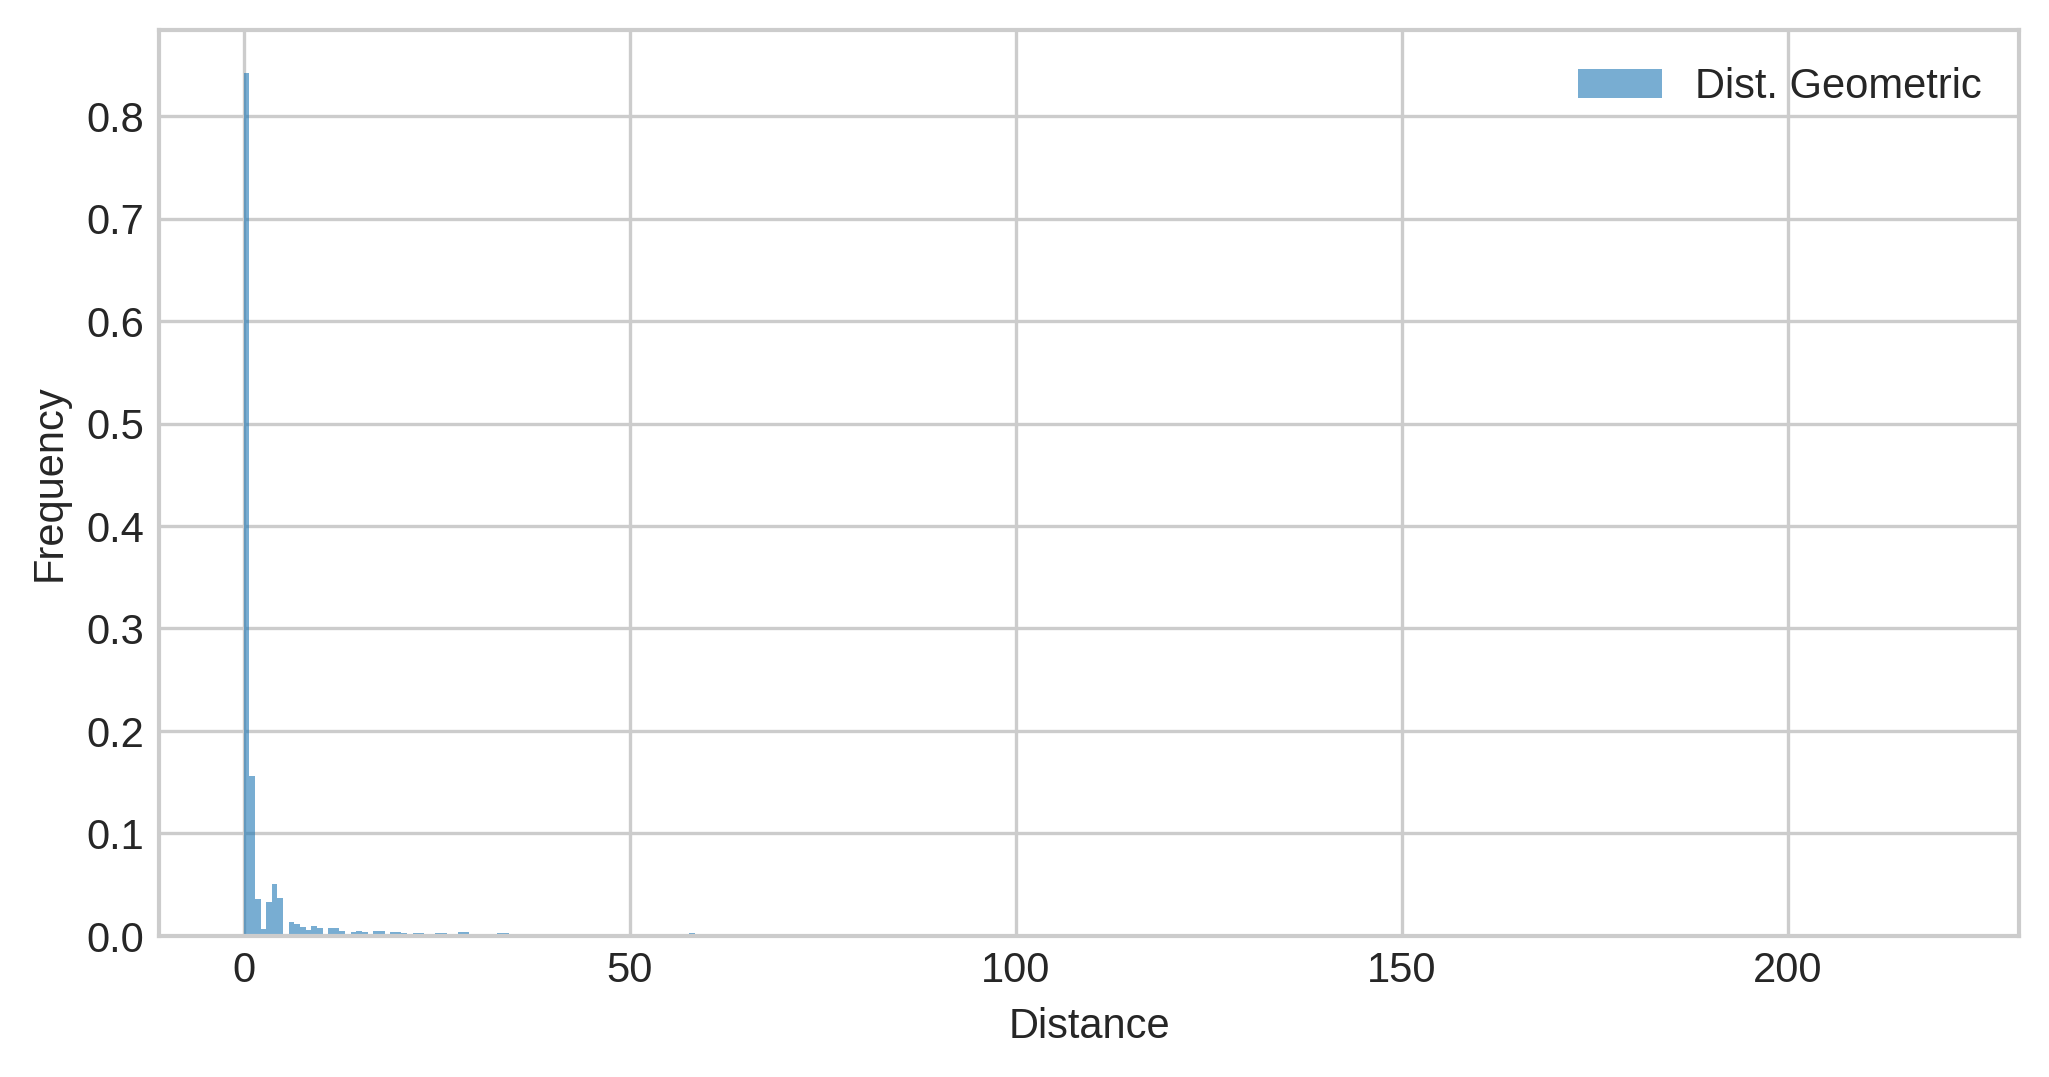
\includegraphics[width=.7\textwidth]{evaluation-results/figures/distance-distr-histogram-full}
    \caption{Full histogram of the distance distribution of the matched segments (binning=300)}
    \label{fig:segment-distance-histogram-full}
\end{figure}

Because of a very long tail, I reduce the further analysis to the distance span between 0 and 40. Figure \ref{fig:segment-distance-distribution} depicts the histogram of distances between matched segments (in 300 bins). It shows that most segments (89\%) are cumulated in first two bins with distance up to 2. The consequent three bins also contain a significant portion of segments with distance up to 5. The rest of the bins, represent a very long tail, spanning on distances up to maximum 219 and containing a small amount of segments. 

\begin{figure}[!ht]
    \centering
    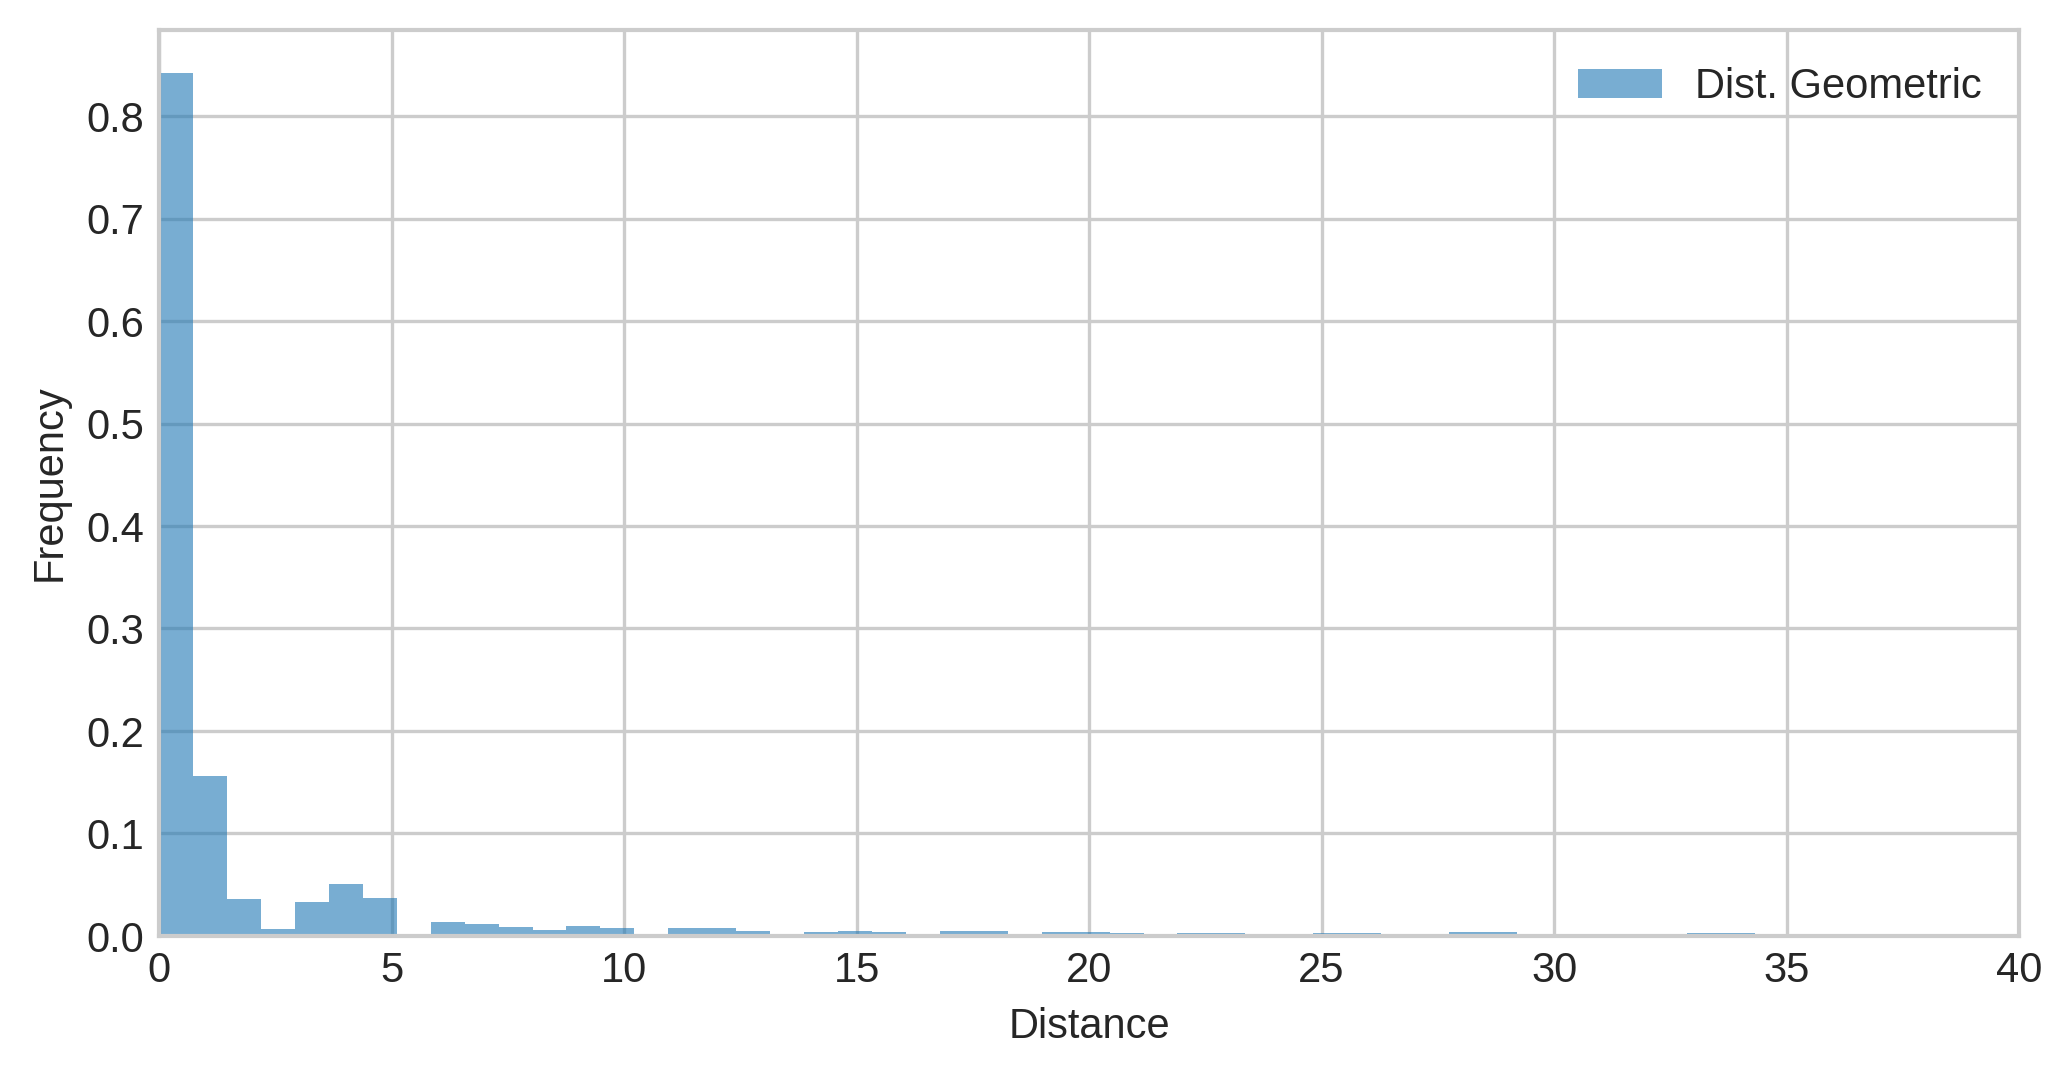
\includegraphics[width=.7\textwidth]{evaluation-results/figures/distance-distr-histogram}
    \caption{Reduced histogram of the distance distribution of the matched segments (binning=300). View reduced to the a distance of 40 characters}
    \label{fig:segment-distance-histogram}
\end{figure}

This distribution can be viewed in it's cumulative form depicted in Figure \ref{fig:segment-distance-distribution}. Here we see that over 51\% of segments are perfectly aligned. 80\% of the segments are slightly shifted up to a distance of maximum 5 characters. This can be explained by differences in (a) punctuation, (b) conjunction and (c)verbal group treatment described above. The next 5\% of the segments are shifted between 5 and 10 characters. The last 10\% cover the heavy shift of distances 20 to 219. This may be due differences in verbal group treatment, subsumed conjuncts (clause and group conjunctions) and erroneous prepositional phrase attachment (treated as Qualifier instead of Complement/Adjunct or vice versa). 

\begin{figure}[!ht]
    \centering
    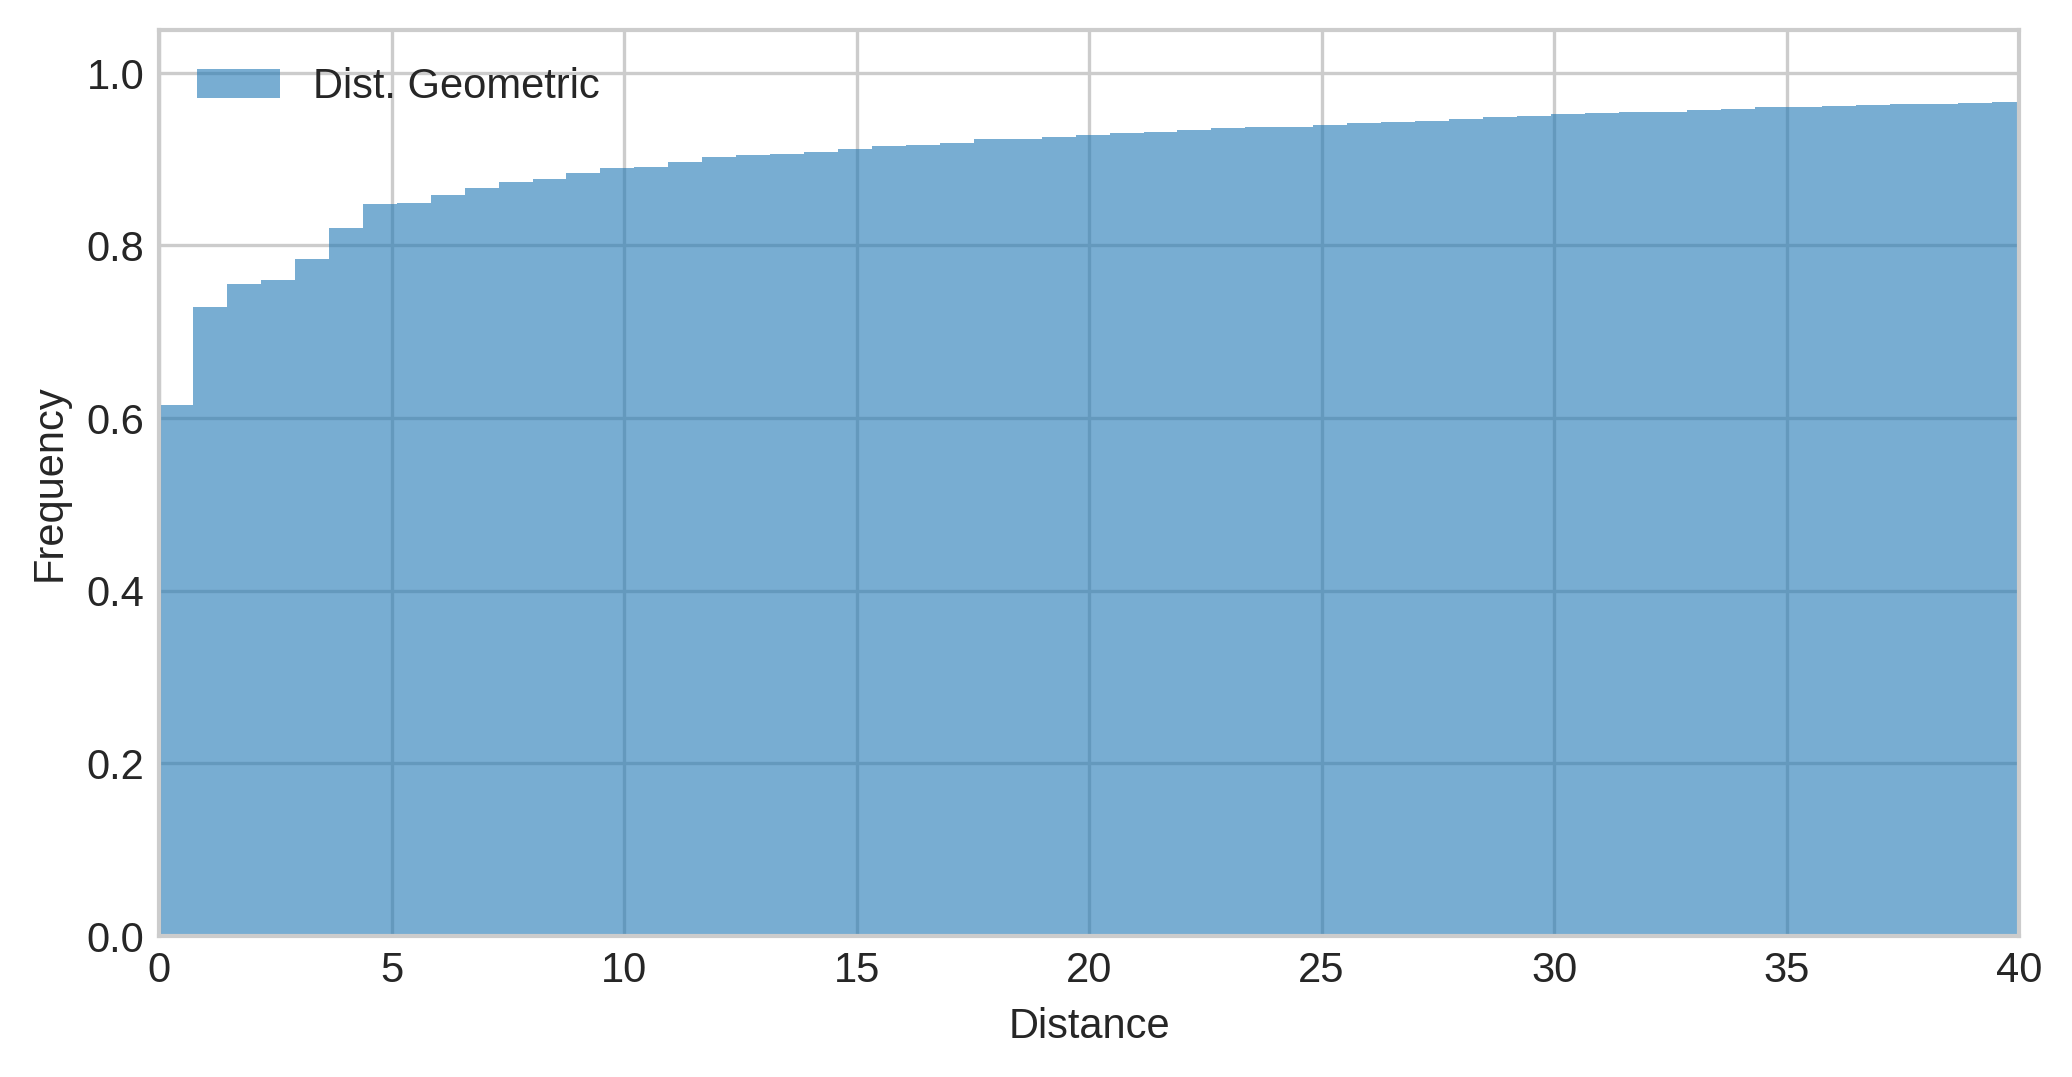
\includegraphics[width=.7\textwidth]{evaluation-results/figures/distance-distr-cumulative}
    \caption{Cumulative histogram of the distance distribution of the matched segments (binning=300). View reduced to the a distance of 40 characters}
    \label{fig:segment-distance-distribution}
\end{figure}

\subsection{Segment divergence breakdown by element type}

If we take a closer look at the Figure \ref{fig:segment-distance-histogram} we will notice some spikes and a tendency towards some local values. What would the histogram look like if we group values in a different manner considering these spikes and the long tail of the distribution. 
In Figure \ref{fig:segment-distance-histogram} we can observe several dips at around distances 3, 6, 11, 13, 17, 19, 22, 24 and so on. I decided to consider these dips for deciding bin borders in the new bin design. And, since the tail is very long with very few values, as the bins advance to the left, each is designed over longer span this way compressing the tail. In Table \ref{tab:progressive-bins} is presented such binning design. Also each interval is assigned a category that means the degree of deviation.

\begin{table}[!ht]
    \begin{tabular}{|c|c|c|c|c|c|c|}
        \hline
        \textbf{degree}          & insignificant & tiny & little & moderate & significant & high   \\ \hline
        \textbf{distance intervals} & 0-3           & 3-5  & 5-10   & 10-20    & 20-50       & 50-250 \\ \hline
    \end{tabular}
    \caption{The progressive binning scale considering the dataset properties}
    \label{tab:progressive-bins}
\end{table}

Besides custom binning described above, looking at each segment label in part brings more clarity to the evaluation. The most relevant segment labels are the unit elements. In the current evaluation, the annotators provide clause level syntactic (subject, complement, adjunct, predicator, finite) and semantic (configuration, main verb, participant) elements. These elements are used a dimension in the breakdown of the segment divergence that follows. 

Using the bins defined in Table \ref{tab:progressive-bins} the distribution of segment deviations grouped by the main syntactic elements is provided in Table \ref{tab:deviation-per-feature-and-degree-constit} that is also depicted in Figure \ref{fig:segment-distance-degree-features-mood}. 

\begin{table}[!ht]
    \begin{tabular}{|c|c|c|c|c|c|c|}
        \hline
        \multirow{2}{*}{\textbf{element}} & \multicolumn{6}{c|}{\textbf{\% of segments per degree of deviation}} \\ \cline{2-7} 
        & \textbf{\begin{tabular}[c]{@{}c@{}}insignificant\\ (0-3)\end{tabular}} & \textbf{\begin{tabular}[c]{@{}c@{}}tiny\\ (3-5)\end{tabular}} & \textbf{\begin{tabular}[c]{@{}c@{}}little\\ (5-10)\end{tabular}} & \textbf{\begin{tabular}[c]{@{}c@{}}moderate\\ (10-20)\end{tabular}} & \textbf{\begin{tabular}[c]{@{}c@{}}significant\\ (20-50)\end{tabular}} & \textbf{\begin{tabular}[c]{@{}c@{}}high\\ (50-250)\end{tabular}} \\ \hline
        predicator & 29.38 & 0.95 & 0.30 & 0.10 & 0.00 & 0.05 \\ \hline
        subject    & 22.70 & 0.10 & 0.25 & 0.30 & 0.05 & 0.00 \\ \hline
        adjunct    & 13.86 & 0.45 & 0.60 & 0.15 & 0.85 & 0.20 \\ \hline
        complement & 12.10 & 0.75 & 1.46 & 2.26 & 1.96 & 1.86 \\ \hline
        finite     & 9.19  & 0.00 & 0.00 & 0.00 & 0.05 & 0.05 \\ \hline
    \end{tabular}
    \caption{Percentage of segments deviated to a given degree for major syntactic elements}
    \label{tab:deviation-per-feature-and-degree-constit}
\end{table}

\begin{figure}[!ht]
    \centering
    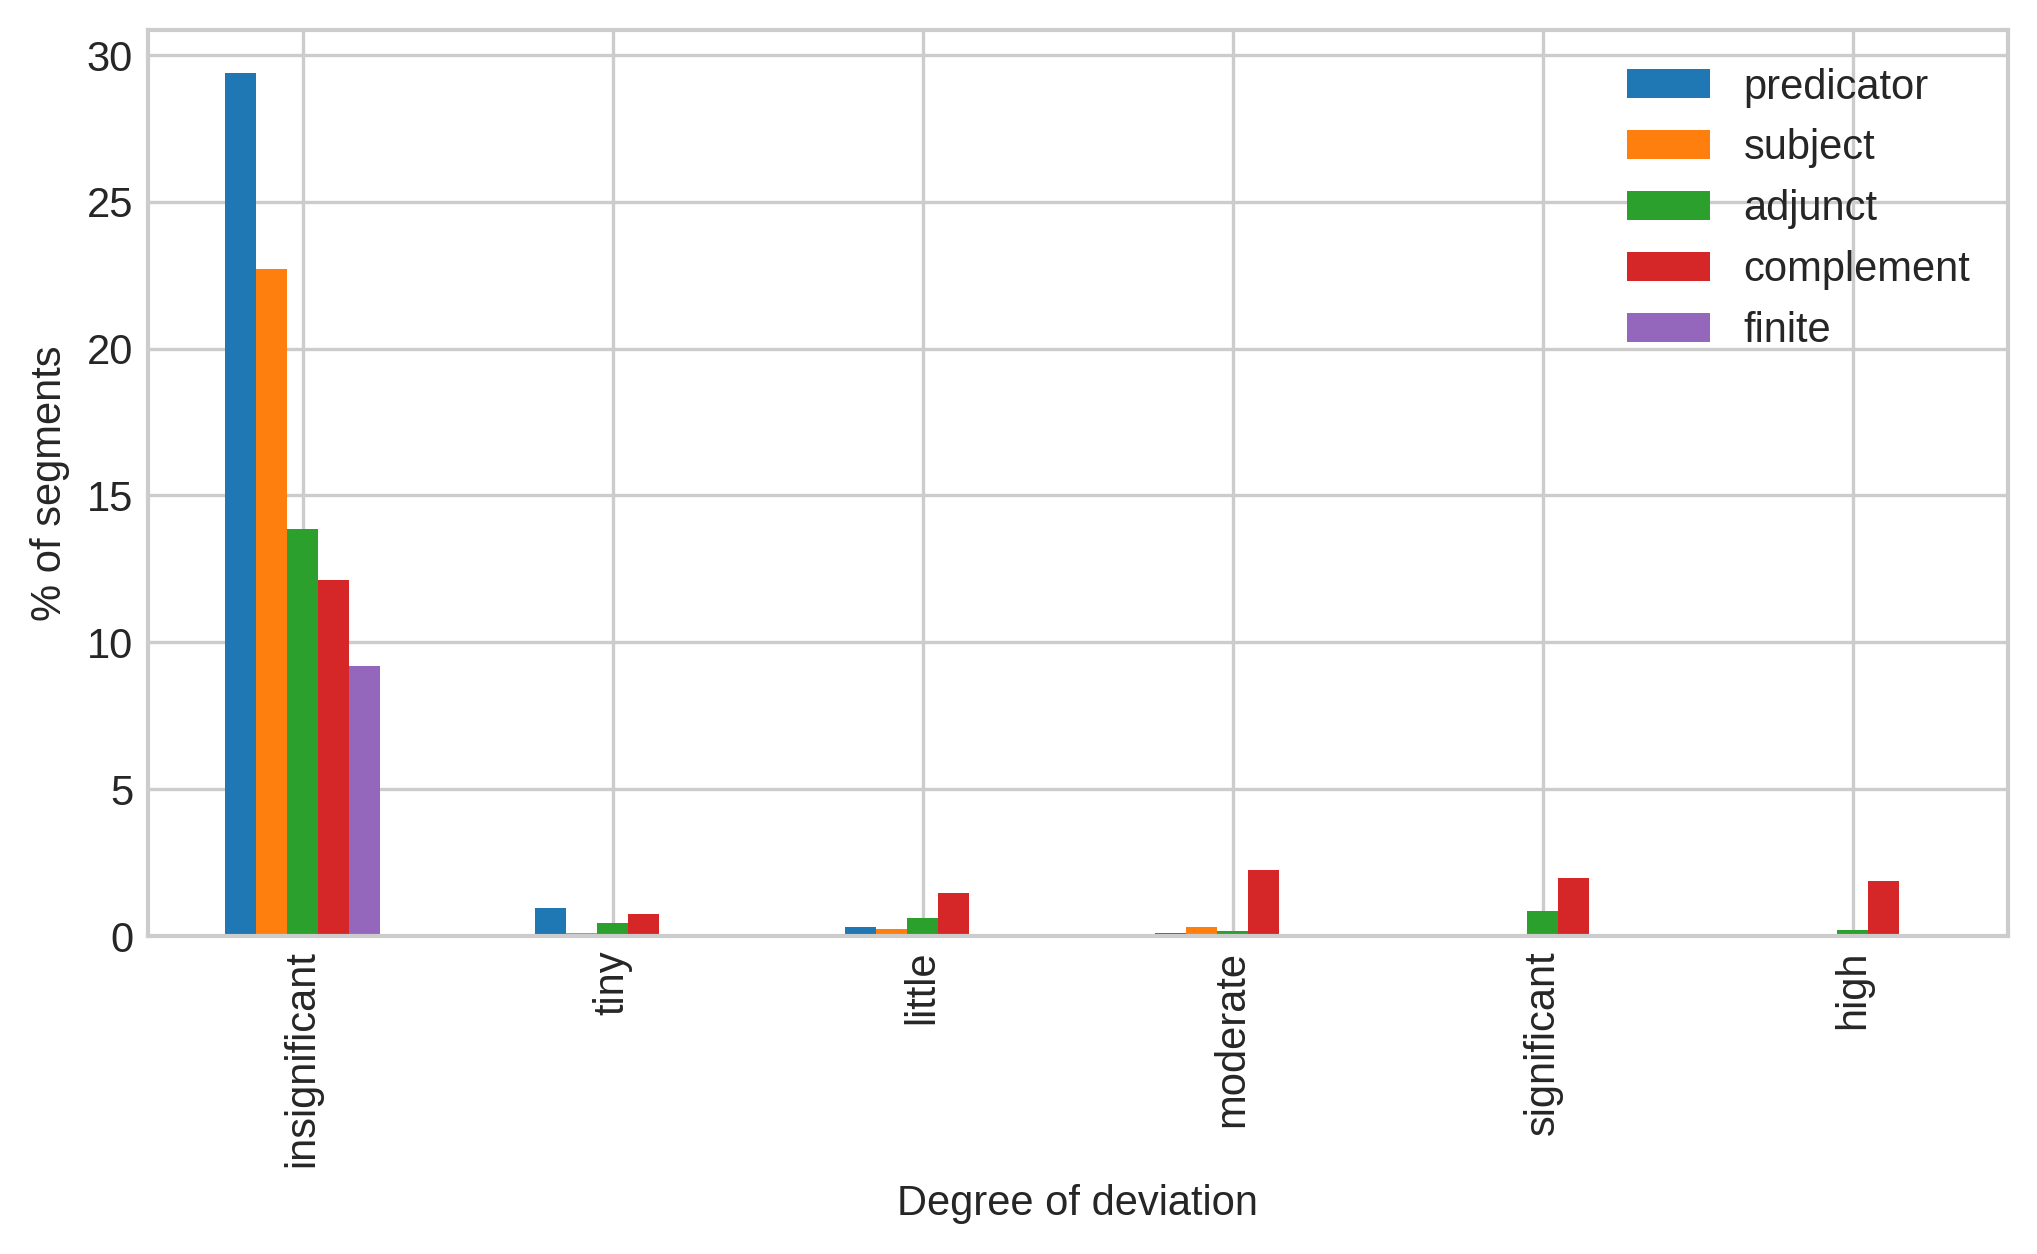
\includegraphics[width=.7\textwidth]{evaluation-results/figures/distance-degree-features-syntactic}
    \caption{Bar chart of the segments deviated to a given degree for major syntactic elements}
    \label{fig:segment-distance-degree-features-mood}
\end{figure}

In Figure \ref{fig:segment-distance-degree-features-mood} we can see that most deviations are insignificant. The number of segments in the rest of the bins, from tiny to high, is below 1\% in every bin which perhaps reflects errors in annotation and/or matching algorithm requiring further investigation. In case of complements, however, the proportion of segments is slightly higher (0.7--2.2\%). This may be explained by the problem of prepositional phrase attachment and further analysis is needed to test this hypothesis. 

When we switch to a grouping by the main Transitivity elements maintaining the same bins defined in Table \ref{tab:progressive-bins}, then the distribution of segment deviations looks as outlined in Table \ref{tab:deviation-per-feature-and-degree-trans}. The same data are depicted in Figure \ref{fig:segment-distance-degree-features-trans}. 

\begin{table}[!ht]
    \begin{tabular}{|c|c|c|c|c|c|c|}
        \hline
        \multirow{2}{*}{\textbf{feature}} & \multicolumn{6}{c|}{\textbf{\% of segments per degree of deviation }}                                                                                                                                                 \\ \cline{2-7} 
        & \textbf{\begin{tabular}[c]{@{}c@{}}insignificant\\ (0-3)\end{tabular}} & \textbf{\begin{tabular}[c]{@{}c@{}}tiny\\ (3-5)\end{tabular}} & \textbf{\begin{tabular}[c]{@{}c@{}}little\\ (5-10)\end{tabular}} & \textbf{\begin{tabular}[c]{@{}c@{}}moderate\\ (10-20)\end{tabular}} & \textbf{\begin{tabular}[c]{@{}c@{}}significant\\ (20-50)\end{tabular}} & \textbf{\begin{tabular}[c]{@{}c@{}}high\\ (50-250)\end{tabular}} \\ \hline
        participant-role & 36.78 & 2.21 & 3.48 & 2.80 & 3.04 & 1.67 \\ \hline
        main             & 20.75 & 3.48 & 1.23 & 0.39 & 0.00 & 0.00 \\ \hline
        configuration    & 7.75  & 3.73 & 2.80 & 3.04 & 4.56 & 2.31 \\ \hline
    \end{tabular}
    \caption{Percentage of segments deviated to a given degree for major semantic elements}
    \label{tab:deviation-per-feature-and-degree-trans}
\end{table}

\begin{figure}[!ht]
    \centering
    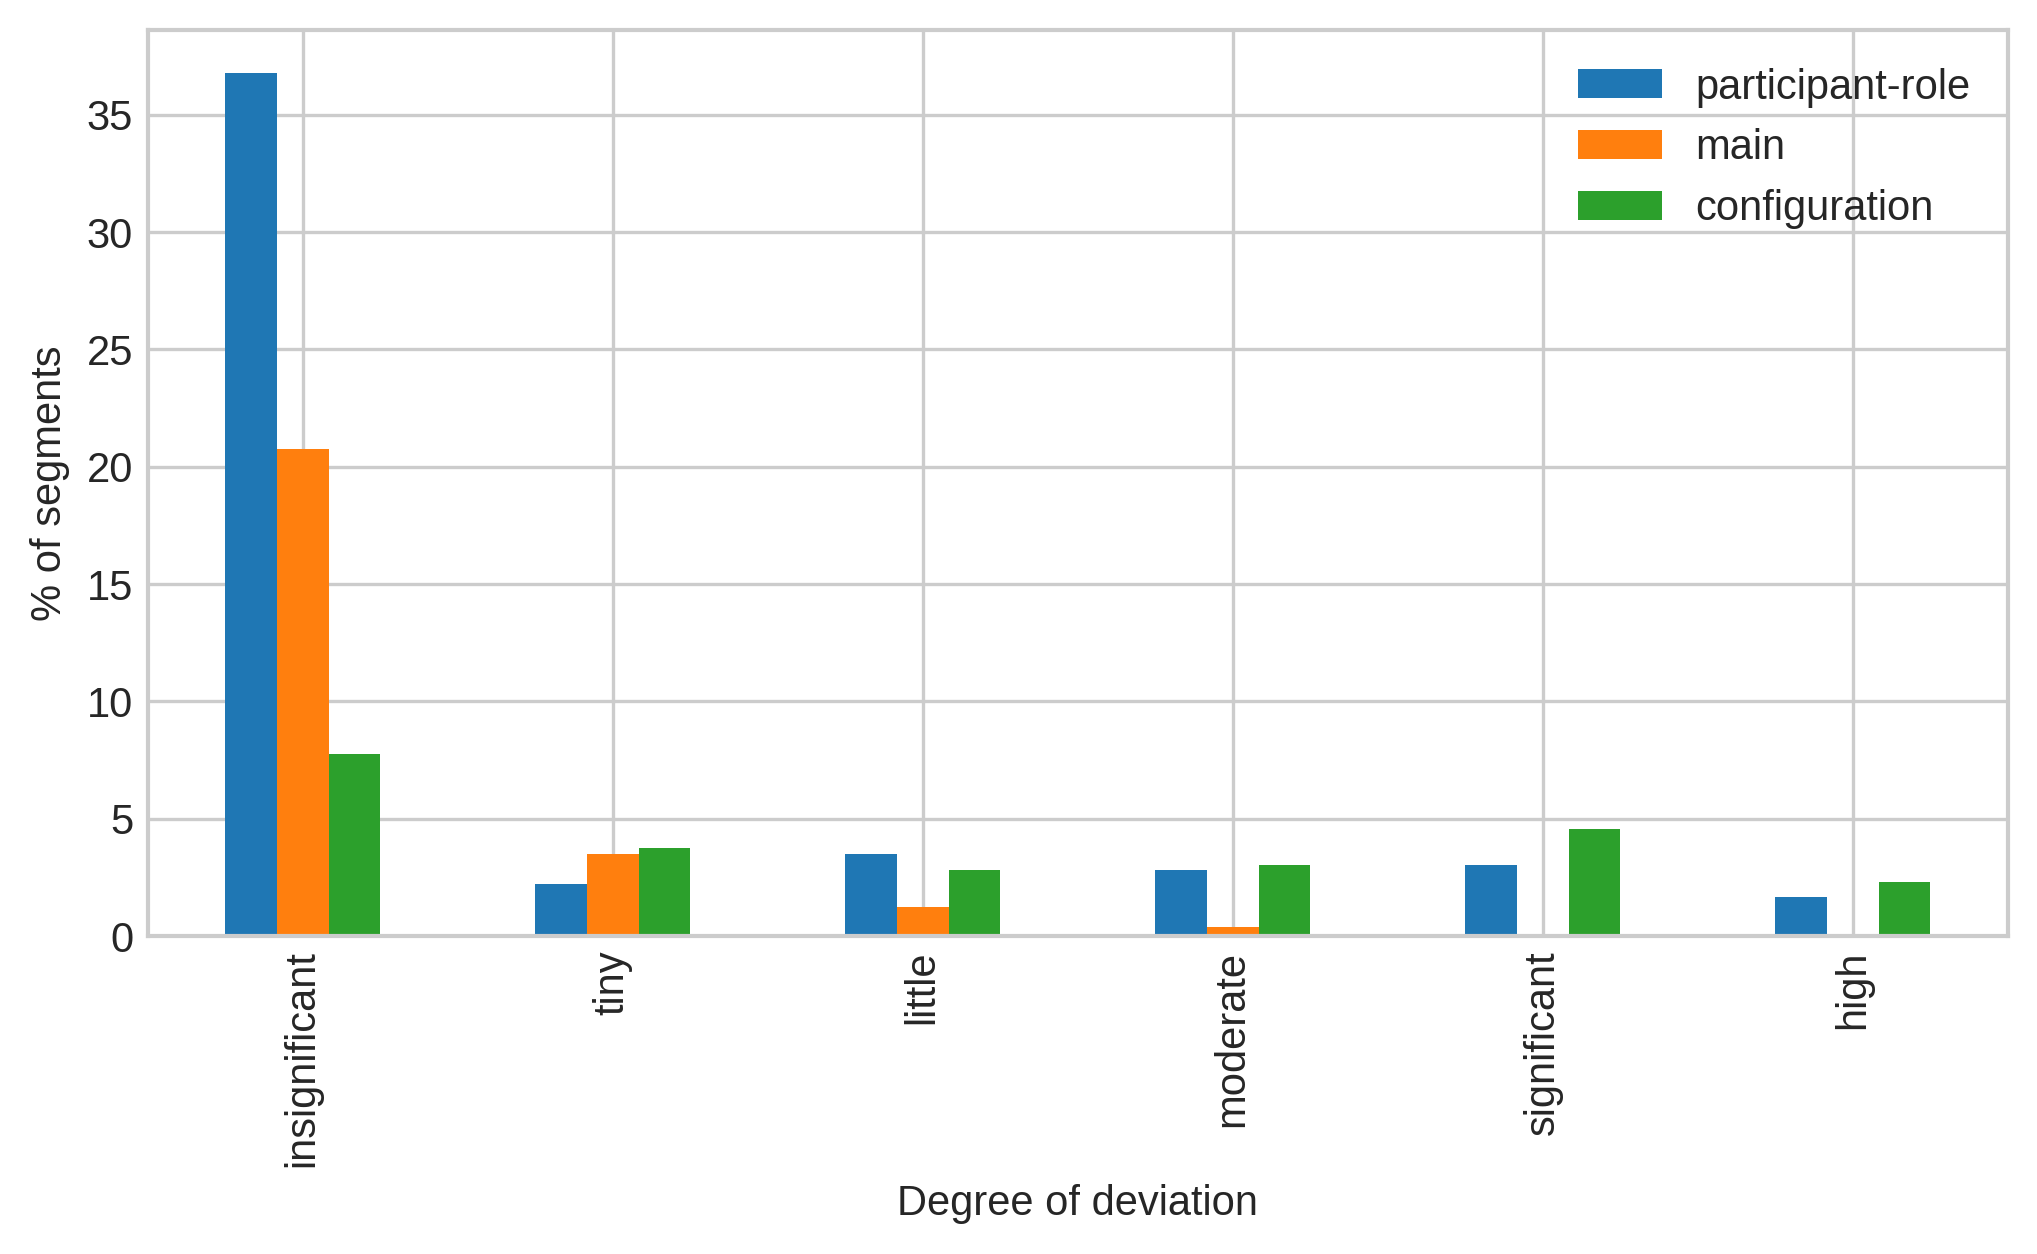
\includegraphics[width=.7\textwidth]{evaluation-results/figures/distance-degree-features-semantic}
    \caption{Bar chart of the feature segments deviated to a given degree for major semantic elements}
    \label{fig:segment-distance-degree-features-trans}
\end{figure}

Similarly to Figure \ref{fig:segment-distance-degree-features-mood}, in Figure \ref{fig:segment-distance-degree-features-trans} we can see that most of the deviations are insignificant (0-3 characters). In the rest of the bins representing higher degrees of deviation the amount of segments is up to 4.7\% which reflects higher number of shifted segments. One exception is the main verb whose occurrences decreases towards higher degrees of deviation, i.e. it is shifted by an insignificant, tiny or little degree that is up to about 10 characters. This is explainable by the fact that the main verb is most of the time (if not always) a single word, which is always shorter than the configuration or participant elements which usually span clauses of groups comprising multiple words. The large variations in participant seems to correlate with complement variation and might be explained by the attachment errors. In cases of high configuration deviation however further investigation are needed because these may possibly be errors in the segment matching algorithm or other unknown anomalies.

\subsection{Syntactic evaluation: Constituency elements}

The evaluation data in this and the following sections will be presented in tables with the same structure. Using Table \ref{tab:constit-unit-types} as example I explain next what the columns mean. The first column will contain the name of the unit type, element or feature. The next three columns \textit{Match}, \textit{Manual mn} and \textit{Parse mn} represent the number of segments that are considered identical between the corpus and parser, the number of unmatched the corpus (manually created) segments and the number of unmatched parser (automatically generated) segments. The next three columns \textit{Precision}, \textit{Recall} and \textit{F_1} represent standard accuracy metrics indicating the fraction of relevant instances among the retrieved instances, fraction of relevant instances that have been retrieved over the total amount of relevant instances and the harmonic mean of the previous two. In addition, the column \textit{\%Total matched} represents the percentage the current item (row) in the table while the \textit{\% Manual nm} and \textit{\%Parse nm} represent the number of remaining unmatched segments of the current item (row) that represents a translation of the Manual and Parse mn columns into relative terms. 

\begin{table}[!ht]
    \resizebox{\textwidth}{!}{%
        \begin{tabular}{|c|c|c|c|c|c|c|c|c|c|}
            \hline
            \textbf{Unit type} & \textbf{Matched} & \textbf{\begin{tabular}[c]{@{}c@{}}Manual \\ nm\end{tabular}} & \textbf{\begin{tabular}[c]{@{}c@{}}Parse \\ nm\end{tabular}} & \textbf{Precision} & \textbf{Recall} & \textbf{F1} & \textbf{\begin{tabular}[c]{@{}c@{}}\%Total \\ matched\end{tabular}} & \textbf{\begin{tabular}[c]{@{}c@{}}\%Manual \\ nm\end{tabular}} & \textbf{\begin{tabular}[c]{@{}c@{}}\%Parse \\ nm\end{tabular}} \\ \hline
            clause              & 612.00 & 64.00  & 78.00  & 0.89 & 0.91 & 0.90 & 37.00 & 9.47  & 11.30 \\ \hline
            nominal-group       & 717.00 & 108.00 & 67.00  & 0.91 & 0.87 & 0.89 & 43.35 & 13.09 & 8.55  \\ \hline
            prepositional-group & 119.00 & 39.00  & 39.00  & 0.75 & 0.75 & 0.75 & 7.19  & 24.68 & 24.68 \\ \hline
            adverbial-group     & 161.00 & 79.00  & 103.00 & 0.61 & 0.67 & 0.64 & 9.73  & 32.92 & 39.02 \\ \hline
            adjectival-group    & 45.00  & 36.00  & 38.00  & 0.54 & 0.56 & 0.55 & 2.72  & 44.44 & 45.78 \\ \hline
        \end{tabular}
    }
    \caption{The evaluation statistics for the main constituency unit types}
    \label{tab:constit-unit-types}
\end{table}

The syntactic accuracy aims to measure how well the main unit types and the clause main elements have been detected by the parsed compared to the corpus. The evaluation is performed on the OCD corpus. This evaluation is restricted to the clause and four group types: nominal, prepositional, adverbial and adjectival. No clause complexes, group complexes or word types are included. The evaluation results are presented in Table \ref{tab:constit-unit-types} where we can see that clauses and nominal groups have an F_1 score of about 90\%. Prepositional, adverbial and adjectival group scores decrease to 55\% and requires investigation of the errors in the parsing and matching algorithms. There is also a contrast in the number of segments, visible in the bar chart from Figure \ref{fig:constit-unit-types}, between the first two element types and the last three with a ratio of one to four or more.

\begin{figure}[!ht]
    \centering
    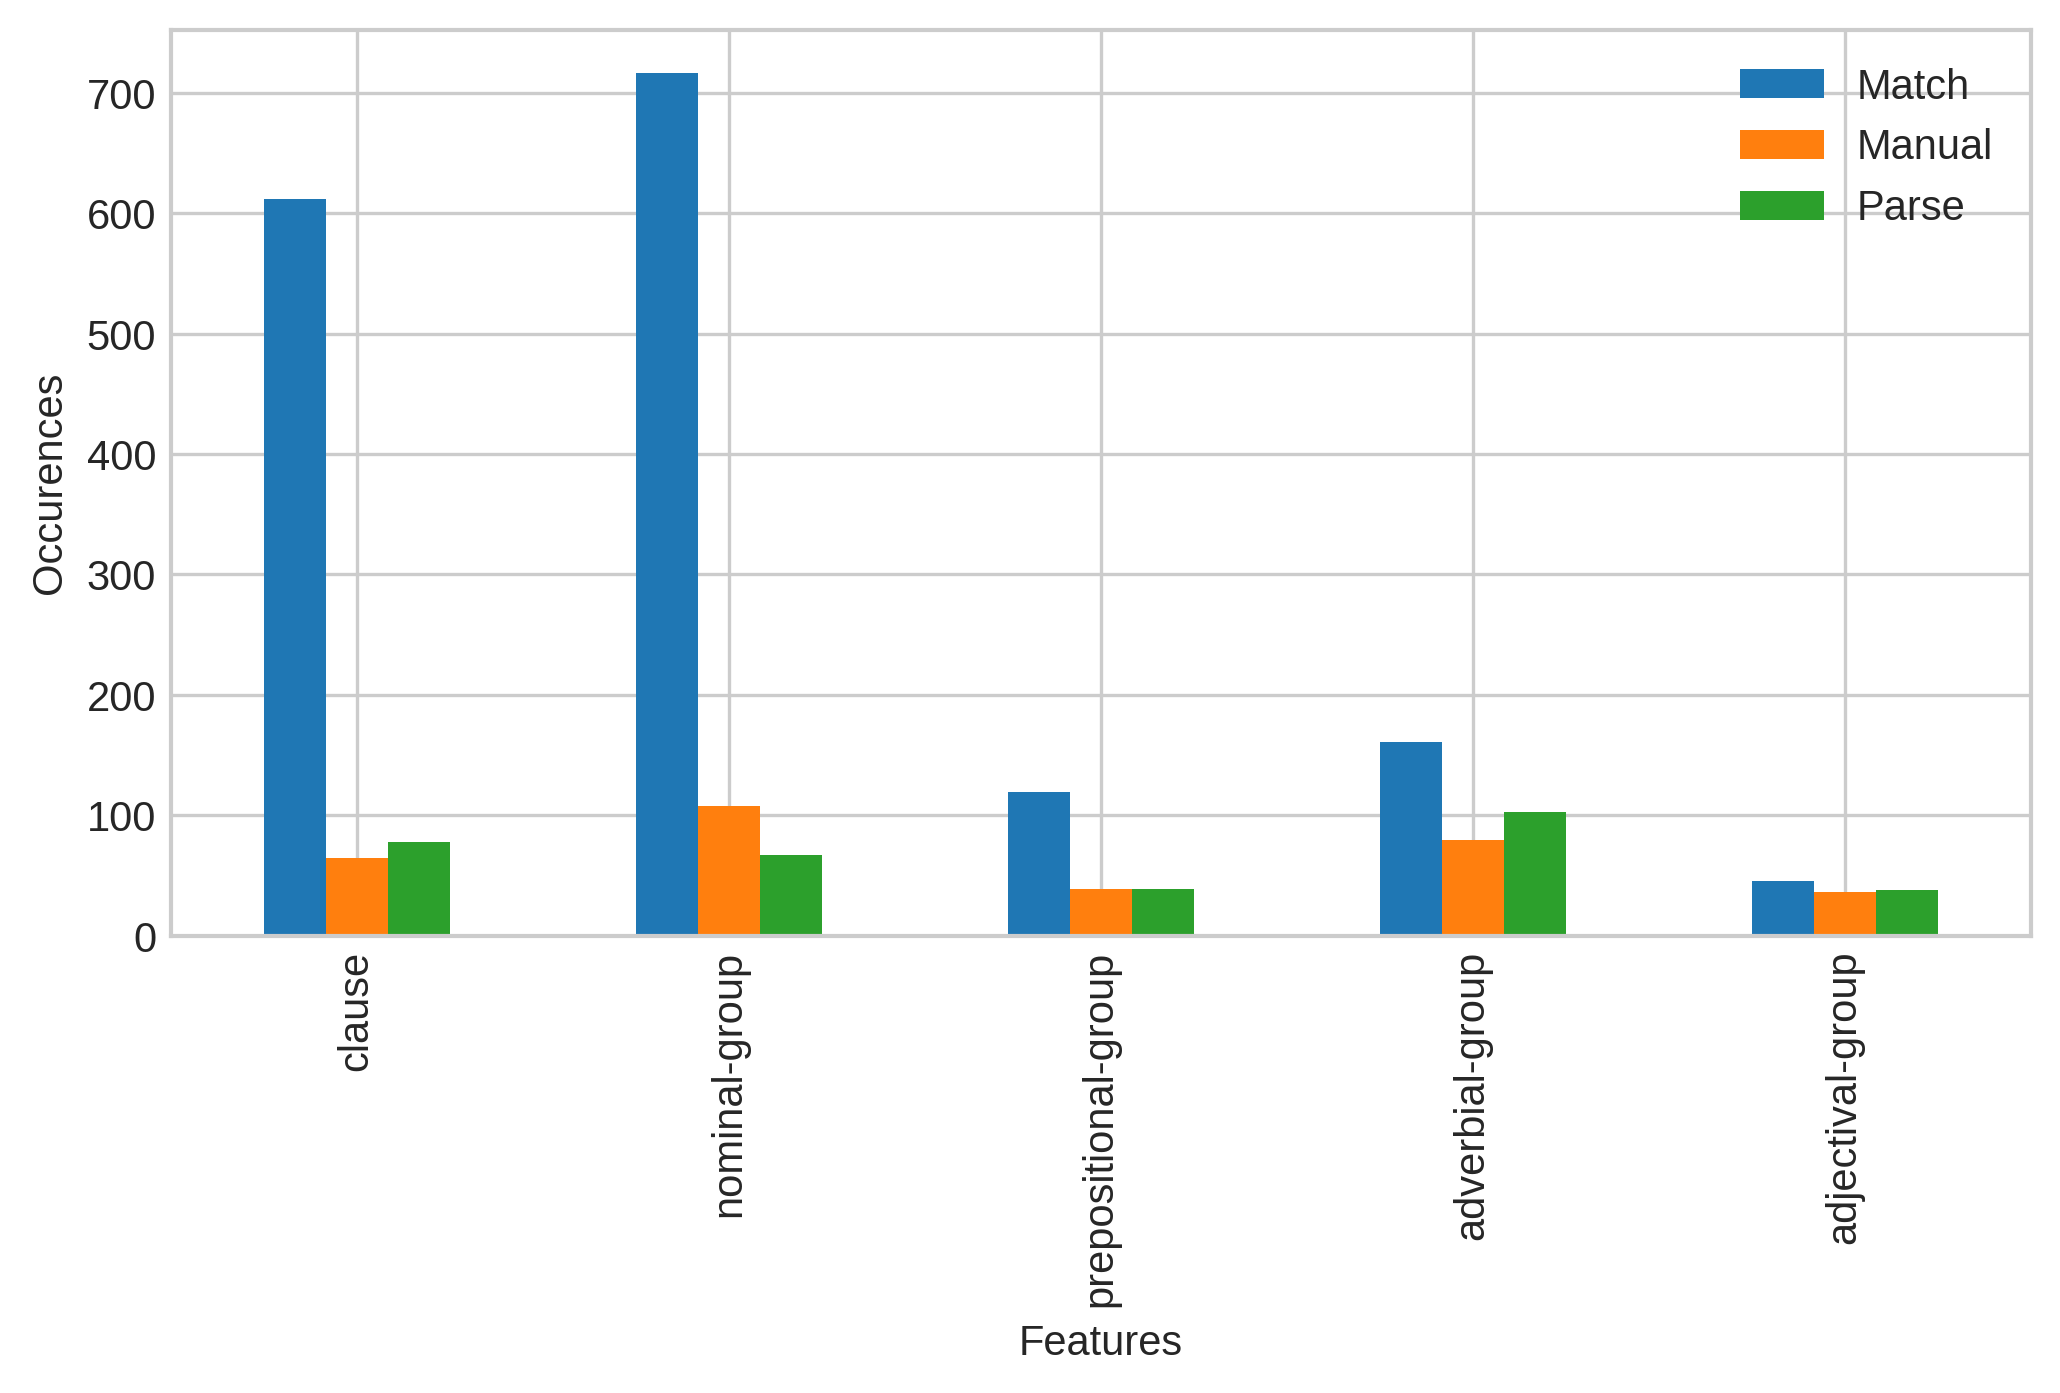
\includegraphics[width=.7\textwidth]{evaluation-results/figures/accuracy-syntactic-group-types}
    \caption{Bar chart of matched and non-matched (manual and parse) segments of the main constituency unit types}
    \label{fig:constit-unit-types}
\end{figure}

Table \ref{tab:constit-unit-elements} presents the evaluation result for the main clause elements. Some of them such as, auxiliary verbs, main verb extension, negation particle, and others have been omitted in the corpus and thus missing in the present evaluation. For the predicator (i.e main verb) and subject elements the F_1 measure raises to 90\%. For the complements and finite the F_1 score is 67\% and 63\%. Surprisingly the complements have a small number of corpus unmatched segments and a high number of parser unmatched segments. This is explained by a flaw in the annotation methodology because the clausal complements were often annotated directly as new clause and omitting to draw the same segment with complement element. This required the corpus revision and correction. Adjuncts however have a higher number of unmatched segments on both sides and this may be dues to bugs in the parser.

\begin{table}[!ht]
    \resizebox{\textwidth}{!}{%
        \begin{tabular}{|c|c|c|c|c|c|c|c|c|c|}
            \hline
            \textbf{Clause element} & \textbf{Matched} & \textbf{\begin{tabular}[c]{@{}c@{}}Manual \\ nm\end{tabular}} & \textbf{\begin{tabular}[c]{@{}c@{}}Parse \\ nm\end{tabular}} & \textbf{Precision} & \textbf{Recall} & \textbf{F1} & \textbf{\begin{tabular}[c]{@{}c@{}}\%Total \\ matched\end{tabular}} & \textbf{\begin{tabular}[c]{@{}c@{}}\%Manual \\ nm\end{tabular}} & \textbf{\begin{tabular}[c]{@{}c@{}}\%Parse \\ nm\end{tabular}} \\ \hline
            predicator & 613 & 60  & 79  & 0.89 & 0.91 & 0.90 & 30.79 & 8.92  & 11.42 \\ \hline
            subject    & 466 & 22  & 86  & 0.84 & 0.95 & 0.90 & 23.41 & 4.51  & 15.58 \\ \hline
            complement & 406 & 43  & 350 & 0.54 & 0.90 & 0.67 & 20.39 & 9.58  & 46.30 \\ \hline
            adjunct    & 321 & 159 & 224 & 0.59 & 0.67 & 0.63 & 16.12 & 33.12 & 41.10 \\ \hline
            finite     & 185 & 3   & 392 & 0.32 & 0.98 & 0.48 & 9.29  & 1.60  & 67.94 \\ \hline
        \end{tabular}
    }
    \caption{The evaluation statistics for the clause main elements}
    \label{tab:constit-unit-elements}
\end{table}

\begin{figure}[!ht]
    \centering
    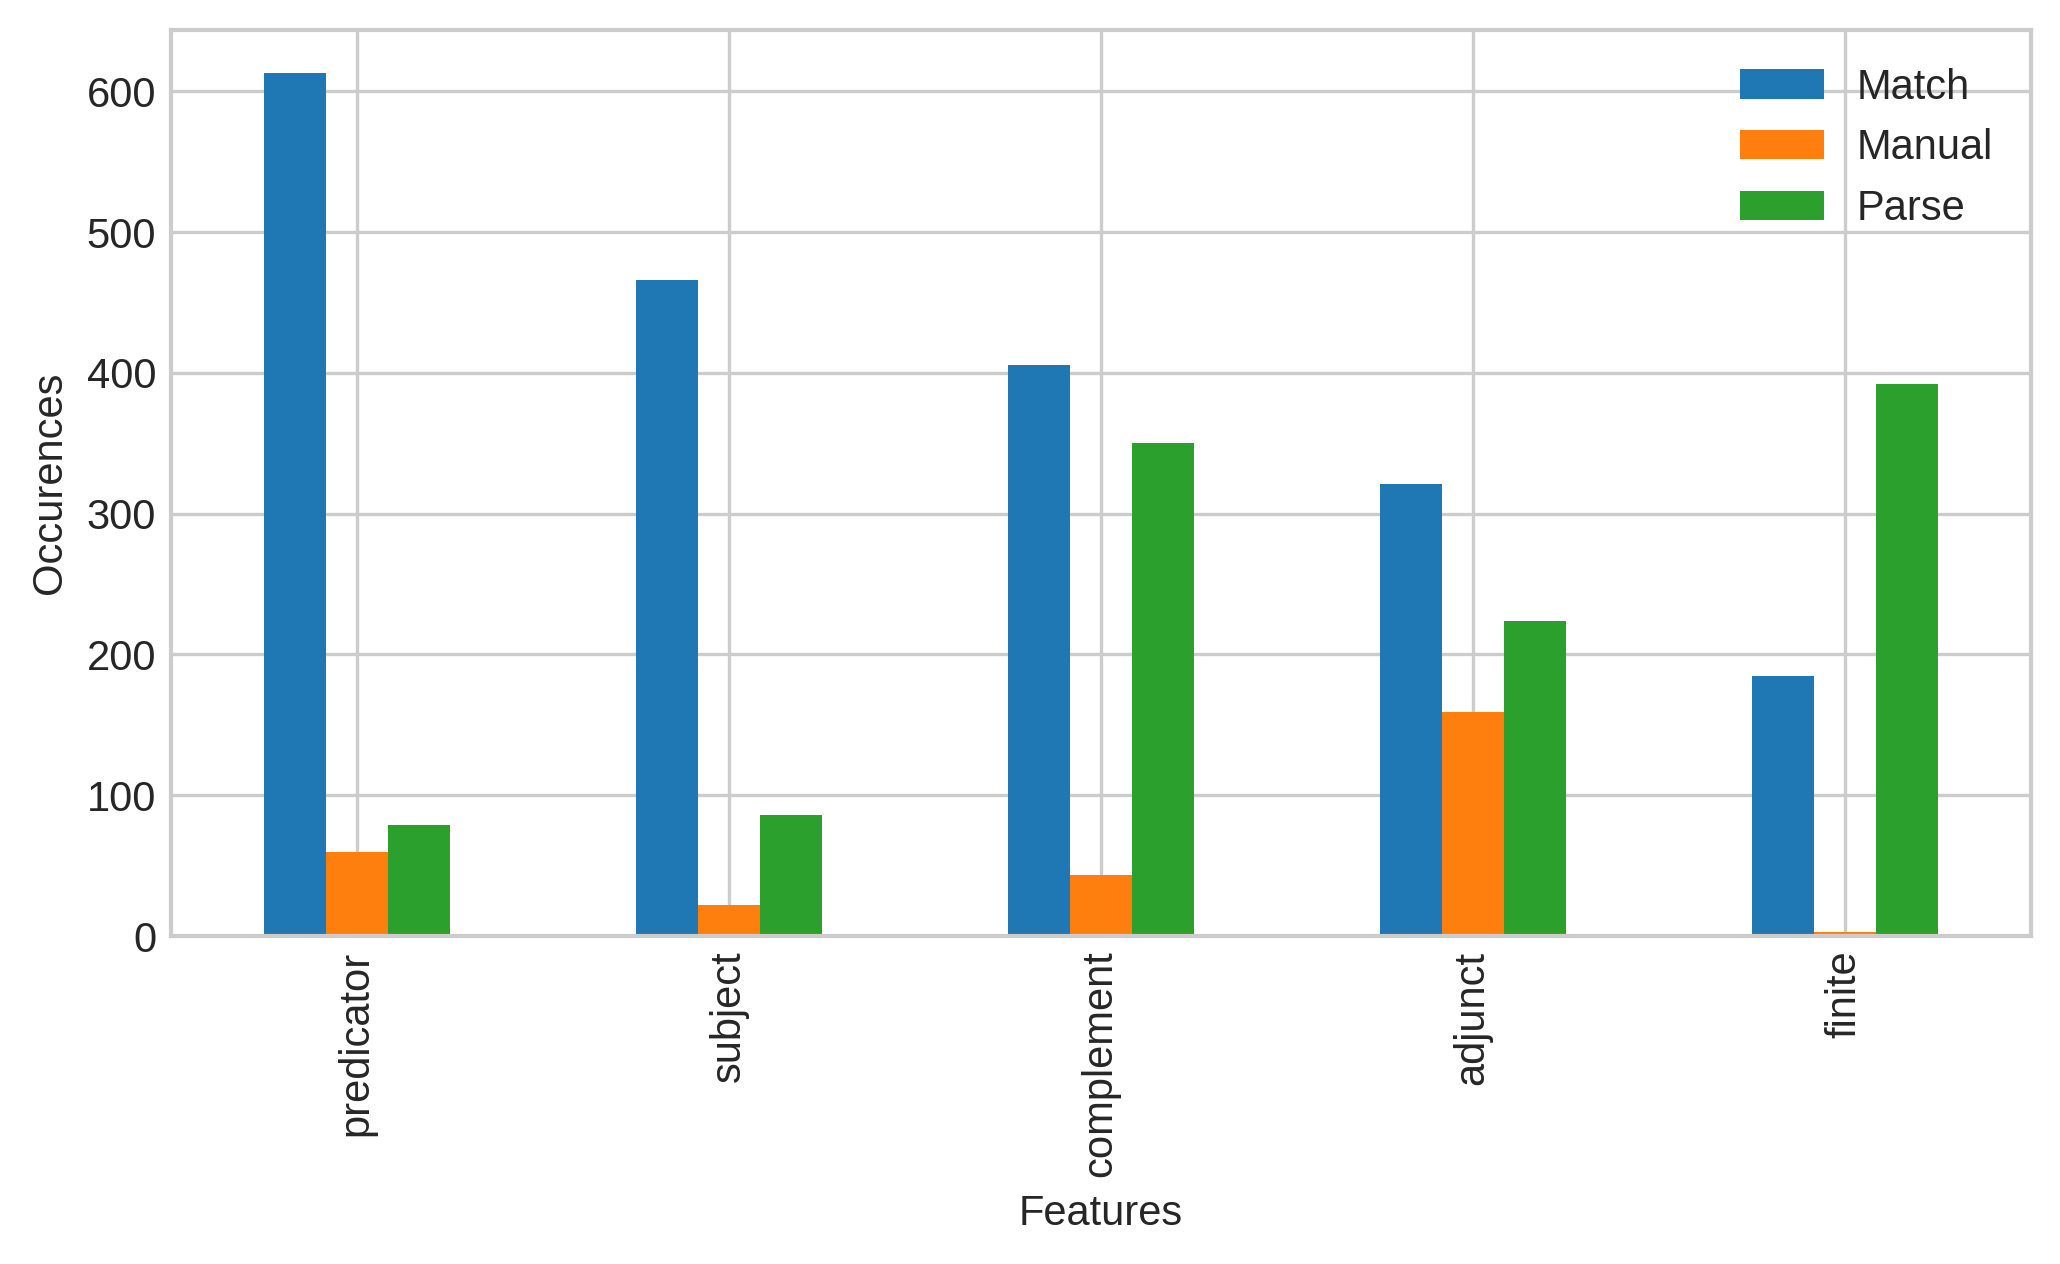
\includegraphics[width=.7\textwidth]{evaluation-results/figures/accuracy-syntactic-clause-elements}
    \caption{Bar chart of matched and non-matched (manual and parse) segments of the clause main elements}
    \label{fig:constit-unit-elements}
\end{figure}

\subsection{Syntactic evaluation: Mood feature selections}
%todo continue here
In this section I present the evaluation of Mood system network selections. The corpus contains selections from a pat of the system network that is depicted in Figure \ref{fig:mood-ocd-simplified}. The full system network is provided in Figure \ref{fig:clause-mood}. Employing the entire system network in the annotations was difficult because as the delicacy increases the time spent for the annotation process increases. 

\begin{figure}[!ht]
    \centering
    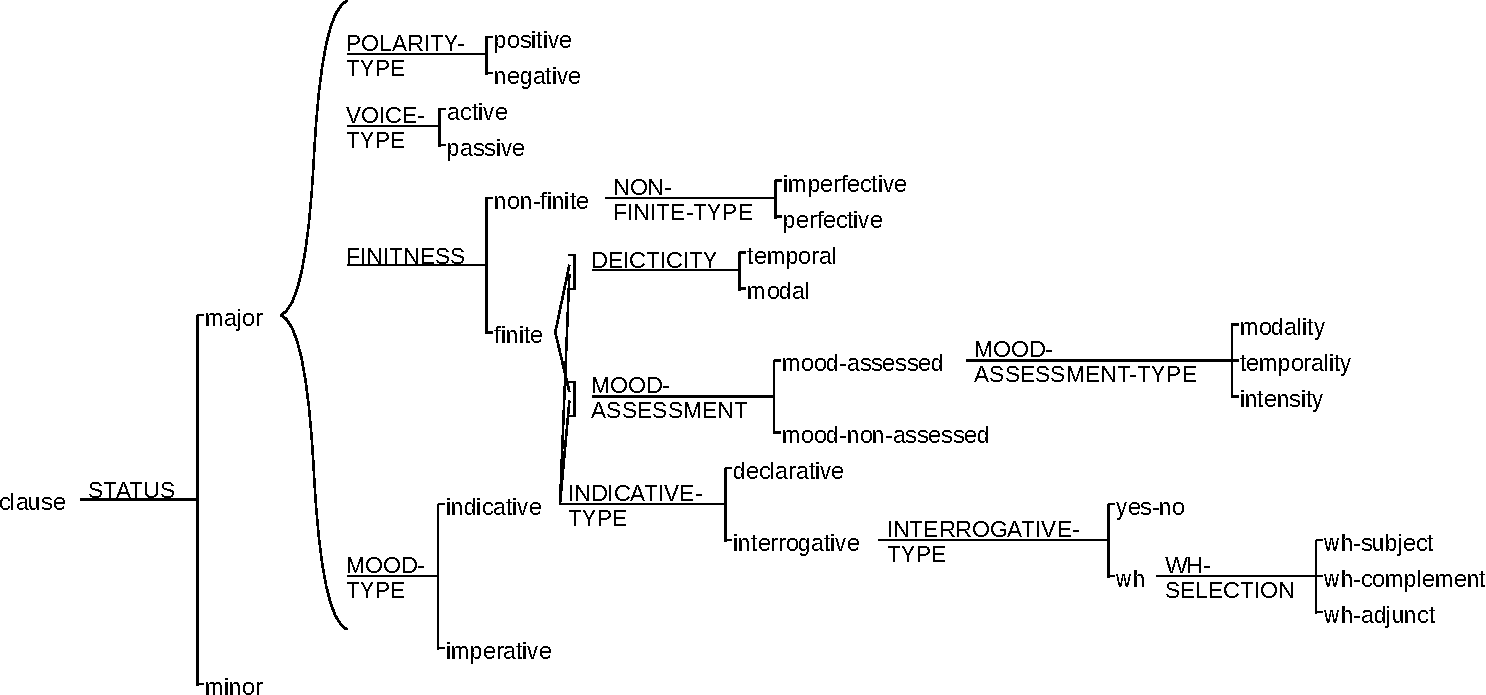
\includegraphics[width=.95\textwidth]{Figures/Evaluation/ocd1-mood-simplified.pdf}
    \caption{The part of the Mood system network that has been used in OCD corpus annotation}
    \label{fig:mood-ocd-simplified}
\end{figure}

\begin{table}[!ht]
    \resizebox{\textwidth}{!}{%
        \begin{tabular}{|c|c|c|c|c|c|c|c|c|c|}
            \hline
            \textbf{Feature} & \textbf{Matched} & \textbf{\begin{tabular}[c]{@{}c@{}}Manual \\ nm\end{tabular}} & \textbf{\begin{tabular}[c]{@{}c@{}}Parse \\ nm\end{tabular}} & \textbf{Precision} & \textbf{Recall} & \textbf{F1} & \textbf{\begin{tabular}[c]{@{}c@{}}\%Total \\ matched\end{tabular}} & \textbf{\begin{tabular}[c]{@{}c@{}}\%Manual \\ nm\end{tabular}} & \textbf{\begin{tabular}[c]{@{}c@{}}\%Parse \\ nm\end{tabular}} \\ \hline
            POLARITY-TYPE &  &  &  &  &  &  &  &  &  \\ \hline
            positive & 485.00 & 125.00 & 55.00 & 0.90 & 0.80 & 0.84 & 89.48 & 20.49 & 10.19 \\ \hline
            negative & 57.00  & 10.00  & 70.00 & 0.45 & 0.85 & 0.59 & 10.52 & 14.93 & 55.12 \\ \hline
            VOICE-TYPE &  &  &  &  &  &  &  &  &  \\ \hline
            active  & 553.00 & 102.00 & 68.00 & 0.89 & 0.84 & 0.87 & 98.05 & 15.57 & 10.95 \\ \hline
            passive & 11.00  & 11.00  & 28.00 & 0.28 & 0.50 & 0.36 & 1.95  & 50.00 & 71.79 \\ \hline
            FINITNESS &  &  &  &  &  &  &  &  &  \\ \hline
            non-finite   & 99.00  & 19.00 & 38.00  & 0.72 & 0.84 & 0.78 & 15.84 & 16.10 & 27.74 \\ \hline
            finite       & 526.00 & 33.00 & 554.00 & 0.49 & 0.94 & 0.64 & 84.16 & 5.90  & 51.30 \\ \hline
            NON-FINITE-TYPE &  &  &  &  &  &  &  &  &  \\ \hline
            perfective   & 71.00  & 12.00 & 16.00  & 0.82 & 0.86 & 0.84 & 73.20 & 14.46 & 18.39 \\ \hline
            imperfective & 26.00  & 9.00  & 24.00  & 0.52 & 0.74 & 0.61 & 26.80 & 25.71 & 48.00 \\ \hline
            DEICTICITY &  &  &  &  &  &  &  &  &  \\ \hline            
            temporal & 446.00 & 74.00 & 55.00 & 0.89 & 0.86 & 0.87 & 97.38 & 14.23 & 10.98 \\ \hline
            modal    & 12.00  & 33.00 & 6.00  & 0.67 & 0.27 & 0.38 & 2.62  & 73.33 & 33.33 \\ \hline
            MOOD-ASSESSMENT-TYPE  &  &  &  &  &  &  &  &  &  \\ \hline            
            temporality & 35.00 & 17.00 & 27.00 & 0.56 & 0.67 & 0.61 & 56.45 & 32.69 & 43.55 \\ \hline
            modality    & 15.00 & 32.00 & 8.00  & 0.65 & 0.32 & 0.43 & 24.19 & 68.09 & 34.78 \\ \hline
            intensity   & 12.00 & 14.00 & 43.00 & 0.22 & 0.46 & 0.30 & 19.35 & 53.85 & 78.18 \\ \hline
            MOOD-TYPE  &  &  &  &  &  &  &  &  &  \\ \hline                        
            indicative    & 455.00 & 216.00 & 37.00 & 0.92 & 0.68 & 0.78 & 99.13 & 32.19 & 7.52  \\ \hline
            imperative    & 4.00   & 1.00   & 31.00 & 0.11 & 0.80 & 0.20 & 0.87  & 20.00 & 88.57 \\ \hline
            INDICATIVE-TYPE  &  &  &  &  &  &  &  &  &  \\ \hline                        
            declarative   & 355.00 & 260.00 & 27.00 & 0.93 & 0.58 & 0.71 & 88.31 & 42.28 & 7.07  \\ \hline
            interrogative & 47.00  & 7.00   & 63.00 & 0.43 & 0.87 & 0.57 & 11.69 & 12.96 & 57.27 \\ \hline
            INTERROGATIVE-TYPE  &  &  &  &  &  &  &  &  &  \\ \hline   
             wh            & 40.00  & 6.00   & 57.00 & 0.41 & 0.87 & 0.56 & 88.89 & 13.04 & 58.76 \\ \hline
            yes-no        & 5.00   & 3.00   & 8.00  & 0.38 & 0.62 & 0.48 & 11.11 & 37.50 & 61.54 \\ \hline                     
            WH-SELECTION  &  &  &  &  &  &  &  &  &  \\ \hline                        
            wh-subject    & 9.00   & 3.00   & 7.00  & 0.56 & 0.75 & 0.64 & 32.14 & 25.00 & 43.75 \\ \hline
            wh-adjunct    & 11.00  & 15.00  & 3.00  & 0.79 & 0.42 & 0.55 & 39.29 & 57.69 & 21.43 \\ \hline
            wh-complement & 8.00   & 0.00   & 62.00 & 0.11 & 1.00 & 0.21 & 28.57 & 0.00  & 88.57 \\ \hline
        \end{tabular}
    }
    \caption{The evaluation statistics for POLARITY-TYPE systemic choices}
    \label{tab:features-mood}
\end{table}

%\begin{table}[!ht]
%    \resizebox{\textwidth}{!}{%
%        \begin{tabular}{|c|c|c|c|c|c|c|c|c|c|}
%            \hline
%            \textbf{Feature} & \textbf{Matched} & \textbf{\begin{tabular}[c]{@{}c@{}}Manual \\ nm\end{tabular}} & \textbf{\begin{tabular}[c]{@{}c@{}}Parse \\ nm\end{tabular}} & \textbf{Precision} & \textbf{Recall} & \textbf{F1} & \textbf{\begin{tabular}[c]{@{}c@{}}\%Total \\ matched\end{tabular}} & \textbf{\begin{tabular}[c]{@{}c@{}}\%Manual \\ nm\end{tabular}} & \textbf{\begin{tabular}[c]{@{}c@{}}\%Parse \\ nm\end{tabular}} \\ \hline
%            positive & 485.00 & 125.00 & 55.00 & 0.90 & 0.80 & 0.84 & 89.48 & 20.49 & 10.19 \\ \hline
%            negative & 57.00  & 10.00  & 70.00 & 0.45 & 0.85 & 0.59 & 10.52 & 14.93 & 55.12 \\ \hline
%        \end{tabular}
%    }
%    \caption{The evaluation statistics for POLARITY-TYPE systemic choices}
%    \label{tab:features-polarity}
%\end{table}

%\begin{table}[!ht]
%    \resizebox{\textwidth}{!}{%
%        \begin{tabular}{|c|c|c|c|c|c|c|c|c|c|}
%            \hline
%            \textbf{Feature} & \textbf{Matched} & \textbf{\begin{tabular}[c]{@{}c@{}}Manual \\ nm\end{tabular}} & \textbf{\begin{tabular}[c]{@{}c@{}}Parse \\ nm\end{tabular}} & \textbf{Precision} & \textbf{Recall} & \textbf{F1} & \textbf{\begin{tabular}[c]{@{}c@{}}\%Total \\ matched\end{tabular}} & \textbf{\begin{tabular}[c]{@{}c@{}}\%Manual \\ nm\end{tabular}} & \textbf{\begin{tabular}[c]{@{}c@{}}\%Parse \\ nm\end{tabular}} \\ \hline
%            active  & 553.00 & 102.00 & 68.00 & 0.89 & 0.84 & 0.87 & 98.05 & 15.57 & 10.95 \\ \hline
%            passive & 11.00  & 11.00  & 28.00 & 0.28 & 0.50 & 0.36 & 1.95  & 50.00 & 71.79 \\ \hline
%        \end{tabular}
%    }
%    \caption{The evaluation statistics for VOICE-TYPE systemic choices}
%    \label{tab:features-voice}
%\end{table}

%\begin{table}[!ht]
%    \resizebox{\textwidth}{!}{%
%        \begin{tabular}{|c|c|c|c|c|c|c|c|c|c|}
%            \hline
%            \textbf{Feature} & \textbf{Matched} & \textbf{\begin{tabular}[c]{@{}c@{}}Manual \\ nm\end{tabular}} & \textbf{\begin{tabular}[c]{@{}c@{}}Parse \\ nm\end{tabular}} & \textbf{Precision} & \textbf{Recall} & \textbf{F1} & \textbf{\begin{tabular}[c]{@{}c@{}}\%Total \\ matched\end{tabular}} & \textbf{\begin{tabular}[c]{@{}c@{}}\%Manual \\ nm\end{tabular}} & \textbf{\begin{tabular}[c]{@{}c@{}}\%Parse \\ nm\end{tabular}} \\ \hline
%            non-finite   & 99.00  & 19.00 & 38.00  & 0.72 & 0.84 & 0.78 & 15.84 & 16.10 & 27.74 \\ \hline
%            finite       & 526.00 & 33.00 & 554.00 & 0.49 & 0.94 & 0.64 & 84.16 & 5.90  & 51.30 \\ \hline
%        \end{tabular}
%    }
%    \caption{The evaluation statistics for FINITNESS systemic choices}
%    \label{tab:features-finitness}
%\end{table}

%\begin{table}[!ht]
%    \resizebox{\textwidth}{!}{%
%        \begin{tabular}{|c|c|c|c|c|c|c|c|c|c|}
%            \hline
%            \textbf{Feature} & \textbf{Matched} & \textbf{\begin{tabular}[c]{@{}c@{}}Manual \\ nm\end{tabular}} & \textbf{\begin{tabular}[c]{@{}c@{}}Parse \\ nm\end{tabular}} & \textbf{Precision} & \textbf{Recall} & \textbf{F1} & \textbf{\begin{tabular}[c]{@{}c@{}}\%Total \\ matched\end{tabular}} & \textbf{\begin{tabular}[c]{@{}c@{}}\%Manual \\ nm\end{tabular}} & \textbf{\begin{tabular}[c]{@{}c@{}}\%Parse \\ nm\end{tabular}} \\ \hline
%            perfective   & 71.00  & 12.00 & 16.00  & 0.82 & 0.86 & 0.84 & 73.20 & 14.46 & 18.39 \\ \hline
%            imperfective & 26.00  & 9.00  & 24.00  & 0.52 & 0.74 & 0.61 & 26.80 & 25.71 & 48.00 \\ \hline
%        \end{tabular}
%    }
%    \caption{The evaluation statistics for NON-FINITE-TYPE systemic choices}
%    \label{tab:features-perfectivity}
%\end{table}

%----deicticity
%\begin{table}[!ht]
%    \resizebox{\textwidth}{!}{%
%        \begin{tabular}{|c|c|c|c|c|c|c|c|c|c|}
%            \hline
%            \textbf{Feature} & \textbf{Matched} & \textbf{\begin{tabular}[c]{@{}c@{}}Manual \\ nm\end{tabular}} & \textbf{\begin{tabular}[c]{@{}c@{}}Parse \\ nm\end{tabular}} & \textbf{Precision} & \textbf{Recall} & \textbf{F1} & \textbf{\begin{tabular}[c]{@{}c@{}}\%Total \\ matched\end{tabular}} & \textbf{\begin{tabular}[c]{@{}c@{}}\%Manual \\ nm\end{tabular}} & \textbf{\begin{tabular}[c]{@{}c@{}}\%Parse \\ nm\end{tabular}} \\ \hline
%            temporal & 446.00 & 74.00 & 55.00 & 0.89 & 0.86 & 0.87 & 97.38 & 14.23 & 10.98 \\ \hline
%            modal    & 12.00  & 33.00 & 6.00  & 0.67 & 0.27 & 0.38 & 2.62  & 73.33 & 33.33 \\ \hline
%        \end{tabular}
%    }
%    \caption{The evaluation statistics for DEICTICITY systemic choices}
%    \label{tab:features-deicticity}
%\end{table}

%----mood assesment
%\begin{table}[]
%    \resizebox{\textwidth}{!}{%
%        \begin{tabular}{|c|c|c|c|c|c|c|c|c|c|}
%            \hline
%            \textbf{Feature} & \textbf{Matched} & \textbf{\begin{tabular}[c]{@{}c@{}}Manual \\ nm\end{tabular}} & \textbf{\begin{tabular}[c]{@{}c@{}}Parse \\ nm\end{tabular}} & \textbf{Precision} & \textbf{Recall} & \textbf{F1} & \textbf{\begin{tabular}[c]{@{}c@{}}\%Total \\ matched\end{tabular}} & \textbf{\begin{tabular}[c]{@{}c@{}}\%Manual \\ nm\end{tabular}} & \textbf{\begin{tabular}[c]{@{}c@{}}\%Parse \\ nm\end{tabular}} \\ \hline
%            temporality & 35.00 & 17.00 & 27.00 & 0.56 & 0.67 & 0.61 & 56.45 & 32.69 & 43.55 \\ \hline
%            modality    & 15.00 & 32.00 & 8.00  & 0.65 & 0.32 & 0.43 & 24.19 & 68.09 & 34.78 \\ \hline
%            intensity   & 12.00 & 14.00 & 43.00 & 0.22 & 0.46 & 0.30 & 19.35 & 53.85 & 78.18 \\ \hline
%        \end{tabular}
%    }
%    \caption{The evaluation statistics for MOOD-ASSESSMENT systemic choices}
%    \label{tab:features-mood-assessment}
%\end{table}

%---mood
%\begin{table}[!ht]
%    \resizebox{\textwidth}{!}{%
%        \begin{tabular}{|c|c|c|c|c|c|c|c|c|c|}
%            \hline
%            \textbf{Feature} & \textbf{Matched} & \textbf{\begin{tabular}[c]{@{}c@{}}Manual \\ nm\end{tabular}} & \textbf{\begin{tabular}[c]{@{}c@{}}Parse \\ nm\end{tabular}} & \textbf{Precision} & \textbf{Recall} & \textbf{F1} & \textbf{\begin{tabular}[c]{@{}c@{}}\%Total \\ matched\end{tabular}} & \textbf{\begin{tabular}[c]{@{}c@{}}\%Manual \\ nm\end{tabular}} & \textbf{\begin{tabular}[c]{@{}c@{}}\%Parse \\ nm\end{tabular}} \\ \hline
%            indicative    & 455.00 & 216.00 & 37.00 & 0.92 & 0.68 & 0.78 & 99.13 & 32.19 & 7.52  \\ \hline
%            imperative    & 4.00   & 1.00   & 31.00 & 0.11 & 0.80 & 0.20 & 0.87  & 20.00 & 88.57 \\ \hline
%        \end{tabular}
%    }
%    \caption{The evaluation statistics for MOOD-TYPE systemic choices}
%    \label{tab:features-mood}
%\end{table}

%\begin{table}[!ht]
%    \resizebox{\textwidth}{!}{%
%        \begin{tabular}{|c|c|c|c|c|c|c|c|c|c|}
%            \hline
%            \textbf{Feature} & \textbf{Matched} & \textbf{\begin{tabular}[c]{@{}c@{}}Manual \\ nm\end{tabular}} & \textbf{\begin{tabular}[c]{@{}c@{}}Parse \\ nm\end{tabular}} & \textbf{Precision} & \textbf{Recall} & \textbf{F1} & \textbf{\begin{tabular}[c]{@{}c@{}}\%Total \\ matched\end{tabular}} & \textbf{\begin{tabular}[c]{@{}c@{}}\%Manual \\ nm\end{tabular}} & \textbf{\begin{tabular}[c]{@{}c@{}}\%Parse \\ nm\end{tabular}} \\ \hline
%            declarative   & 355.00 & 260.00 & 27.00 & 0.93 & 0.58 & 0.71 & 88.31 & 42.28 & 7.07  \\ \hline
%            interrogative & 47.00  & 7.00   & 63.00 & 0.43 & 0.87 & 0.57 & 11.69 & 12.96 & 57.27 \\ \hline
%        \end{tabular}
%    }
%    \caption{The evaluation statistics for INDICATIVE-TYPE systemic choices}
%    \label{tab:features-mood1}
%\end{table}

%\begin{table}[!ht]
%    \resizebox{\textwidth}{!}{%
%        \begin{tabular}{|c|c|c|c|c|c|c|c|c|c|}
%            \hline
%            \textbf{Feature} & \textbf{Matched} & \textbf{\begin{tabular}[c]{@{}c@{}}Manual \\ nm\end{tabular}} & \textbf{\begin{tabular}[c]{@{}c@{}}Parse \\ nm\end{tabular}} & \textbf{Precision} & \textbf{Recall} & \textbf{F1} & \textbf{\begin{tabular}[c]{@{}c@{}}\%Total \\ matched\end{tabular}} & \textbf{\begin{tabular}[c]{@{}c@{}}\%Manual \\ nm\end{tabular}} & \textbf{\begin{tabular}[c]{@{}c@{}}\%Parse \\ nm\end{tabular}} \\ \hline
%            wh            & 40.00  & 6.00   & 57.00 & 0.41 & 0.87 & 0.56 & 88.89 & 13.04 & 58.76 \\ \hline
%            yes-no        & 5.00   & 3.00   & 8.00  & 0.38 & 0.62 & 0.48 & 11.11 & 37.50 & 61.54 \\ \hline
%        \end{tabular}
%    }
%    \caption{The evaluation statistics for INTERROGATIVE-TYPE systemic choices}
%    \label{tab:features-mood2}
%\end{table}

%\begin{table}[!ht]
%    \resizebox{\textwidth}{!}{%
%        \begin{tabular}{|c|c|c|c|c|c|c|c|c|c|}
%            \hline
%            \textbf{Feature} & \textbf{Matched} & \textbf{\begin{tabular}[c]{@{}c@{}}Manual \\ nm\end{tabular}} & \textbf{\begin{tabular}[c]{@{}c@{}}Parse \\ nm\end{tabular}} & \textbf{Precision} & \textbf{Recall} & \textbf{F1} & \textbf{\begin{tabular}[c]{@{}c@{}}\%Total \\ matched\end{tabular}} & \textbf{\begin{tabular}[c]{@{}c@{}}\%Manual \\ nm\end{tabular}} & \textbf{\begin{tabular}[c]{@{}c@{}}\%Parse \\ nm\end{tabular}} \\ \hline
%            wh-subject    & 9.00   & 3.00   & 7.00  & 0.56 & 0.75 & 0.64 & 32.14 & 25.00 & 43.75 \\ \hline
%            wh-adjunct    & 11.00  & 15.00  & 3.00  & 0.79 & 0.42 & 0.55 & 39.29 & 57.69 & 21.43 \\ \hline
%            wh-complement & 8.00   & 0.00   & 62.00 & 0.11 & 1.00 & 0.21 & 28.57 & 0.00  & 88.57 \\ \hline
%        \end{tabular}
%    }
%    \caption{The evaluation statistics for WH-SELECTION systemic choices}
%    \label{tab:features-mood3}
%\end{table}

Table \ref{tab:features-mood} summarises the evaluation results for MOOD system network features grouped by system names (in capital). Let me draw your attention to the POLARITY TYPE system where positive polarity scores 84\% F_1 measure and negative one almost 60\%. The positive polarity score is high but intuitively I would have expected even higher score because the polarity of an English clause is positive by default unless a negation marker is found and this represents only 10\% of the clauses in  the corpus. This may be explained however, as a consequence of low delicacy in the parsing algorithm. Current implementation determines polarity by checking for the presence of the negation verbal marker only. Nonetheless a more delicate polarity testing will have to take into consideration polarity indicators from the subject, complement and adjuncts of various type. 

The VOICE-TYPE system has a similar detection mechanism as the polarity. The parser checks whether there is a passive marker in the clause otherwise the active voice is selected. The positive one scores a high F_1 measure (87\%) yet the negative one performs worse than a random classifier.

\subsection{Semantic evaluation: Constituency elements}

This section describes the empirical evaluation of the semantic annotations. This evaluation is based on the OE1 and BTC corpora created by Anke Schultz for her PhD project. She annotated the text with Cardiff Transitivity system.

\subsection{Semantic evaluation: Transitivity feature selections}


%Figure \ref{fig:segment-distance-distribution} represents a cumulative distribution of matches according to the distance. 
%The figure is Because of the long tail of the distribution 
%
% 68\% of the segments have identical spans while the rest of 32\% have minor to major differences of which 19\% are distanced 1-5 characters due to differences in (a) punctuation, (b) conjunction and (c)verbal group treatment described above. The rest 9.9\% of long and very long distances (6-182 characters) are due to differences in verbal group treatment, subsumed conjuncts (clause and group conjunctions) and erroneous prepositional phrase attachment (treated as Qualifier instead of Complement/Adjunct or vice versa).

%\begin{figure}[!ht]
%    \centering
%    \begin{tikzpicture}[pattern-node] 
%    \begin{axis}[
%    scale only axis,
%    axis y line*=left,
%    axis x line*=bottom,
%    xlabel=$Geometric Distance$,
%    ylabel=$Count$,
%    ylabel near ticks,
%    xlabel near ticks]
%    \addplot[color=black, mark = x] coordinates {
%        (0,	3433)
%        (5,	919)
%        (10,	135)
%        (15,	74)
%        (20,	50)
%        (25,	33)
%        (30,	33)
%        (35,	27)
%        (40,	21)
%        (45,	24)
%        (50,	9)
%        (55,	11)
%        (60,	15)
%        (65,	8)
%        (70,	15)
%        (75,	3)
%        (80,18)
%    };
%    \end{axis}
%    
%    \begin{axis}[
%    scale only axis,
%    axis y line*=right,
%    hide x axis,
%    ylabel=$Distribution$,
%    ylabel near ticks]
%    \addplot[color=black, mark = x] coordinates {		
%        (0,		.7110604805)
%        (5,		.1903479702)
%        (10,	.02796188898)
%        (15,	.01532725766)
%        (20,	.01035625518)
%        (25,	.00683512842)
%        (30,	.00683512842)
%        (35,	.0055923778)
%        (40,	.00434962717)
%        (45,	.00497100249)
%        (50,	.00186412593)
%        (55,	.00227837614)
%        (60,	.00310687655)
%        (65,	.00165700083)
%        (70,	.00310687655)
%        (75,	.00062137531)
%        (80,	.00372825186)
%    };
%    \end{axis}
%    \end{tikzpicture}
%    \caption{Segment distance distribution}
%    \label{fig:segment-distance-distribution}
%\end{figure}

%Because the problem formulation slightly differs from the standard one I have implemented the Gale-Shapley algorithm \citep{Gale1962} one of the most efficient algorithms with the corresponding extra requirements.

%The featurered statistics
%
%Next I present evaluation data for systemic features and systems overall annotated in the corpus and parser. In the tables below are presented the following statistics for features and systems (in upper caps): number of segments in corpus containing the feature (M/N) percentage of the in corpus (M/\%), number of segments generated by the parser (A/N) and corresponding percentage (A/\%), precision, recall and F_{1} measures. 
%
%Table \ref{tab:rank-statistics} contains evaluation statistics for the rank system. In this evaluation only group and clause level features have been taken into account excluding those at the word rank which are missing in the corpus. Clause and group constituents are identified with 0.88 and 0.9 F_{1} scores. 

%The marker feature is used for functional words such as prepositions, verbal prepositional particles, coordinating and subordinations conjunctions. However the prepositional phrases in the corpus do not contain the marker segment as the parser generates and only conjunctions and verbal particles are marked leading to low precision of 0.38. Overall the rank constituents are identified with 0.82 F_{1} score.

%\begin{table}[H]
%    \centering
%    \begin{tabulary}{\linewidth}{|L|l|l|l|l|l|l|l|}
%        \hline
%        \textit{Name} & \textit{M/N} & \textit{M/\%} & \textit{A/N} & \textit{A/\%} & \textit{Prec} & \textit{Rec} & \textit{F_{1}} \\ \hline
%        %&                &                 &                 &                  &                    &                 &             \\ \hline
%        RANK          & 2455       & 26.922          & 4052        & 36.156           & 0.716              & 0.902           & 0.762       \\ \hline
%        clause        & 529        & 21.548          & 545         & 13.450           & 
%        0.875              & 0.902           & 0.888       \\ \hline
%        group         & 1699       & 69.206          & 1760        & 43.435           & 0.886              & 0.918           & 0.902       \\ \hline
%        marker        & 224        & 9.124           & 396         & 9.773            & 0.389              & 0.688           & 0.497       \\ \hline
%        word          & 3          & 0.122           & 1351        & 33.342           & -              & -           & -      \\ \hline
%    \end{tabulary}
%    \caption{Rank system evaluation statistics}
%    \label{tab:rank-statistics}
%\end{table}
%
%The clause elements are systematized in Interpersonal function system whose evaluation statistics are contained in the Table \ref{tab:interpersonal-statistics}. Subjects and Predicators have the highest F_{1} scores of 0.889 and 0.888. Indirect objects have been perfectly identified but they are very few and do not have a statistical significance. Adjuncts and Complements (direct objects) have a lower precision and higher recall scoring 0.628 and 0.661 F_{1}. This is in part due to the fact that the parser annotates prepositional phrases that follow a predicate as both Complement and Adjunct being unable to syntactically distinguish between the two and this task being overtaken during the semantic analysis. The Finite elements are distinguished in the corpus only when they stand alone thus are not conflated with the predicator as in Example \ref{ex:non-conflated-finite}. But when the finite is conflated with the Predicator as in Example \ref{ex:conflated-finite} it has not been annotated in the corpus but it should be and further corrections of the corpus shall be implemented. For this reason there is a big difference between precision and recall 0.172 and 0.980 because most Finites in corpus have been identified by the parser and most of them are missing from the corpus. 
%
%\begin{exe}
%    \ex \label{ex:non-conflated-finite} He may (Finite) go (Predicator) home latter.
%    \ex \label{ex:conflated-finite} He already went (Finite/Predicator) home. 
%\end{exe}
%
%\begin{table}[H]
%    \centering
%    \begin{tabulary}{\linewidth}{|L|l|l|l|l|l|l|l|}
%        \hline
%        \textit{Name}          & \textit{M/N} & \textit{M/\%} & \textit{A/N} & \textit{A/\%} & \textit{Prec} & \textit{Rec} & \textit{F_{1}} \\ \hline
%        %&                &                 &                 &                  &                    &                 &             \\ \hline
%        INTERPERSONAL-FUNCTION & 1681       & 18.434          & 2793        & 24.922           & 0.659              & 0.910           & 0.726       \\ \hline
%        finite                 & 150        & 8.923           & 855         & 30.612           & 0.172              & 0.980           & 0.293       \\ \hline
%        adjunct                & 266        & 15.824          & 358         & 12.818           & 0.547              & 0.737           & 0.628       \\ \hline
%        subject                & 389        & 23.141          & 439         & 15.718           & 0.838              & 0.946           & 0.889       \\ \hline
%        complement-direct      & 347        & 20.642          & 594         & 21.267           & 0.524              & 0.896           & 0.661       \\ \hline
%        complement-indirect    & 2          & 0.119           & 2           & 0.072            & 1              & 1           & 1      \\ \hline
%        predicator             & 527        & 31.350          & 545         & 19.513           & 0.873              & 0.903           & 0.888       \\ \hline
%    \end{tabulary}
%    \caption{Mood clause elements evaluation statistics}
%    \label{tab:interpersonal-statistics}
%\end{table}
%
%In Table \ref{tab:group-type-statistics} are presented evaluation statistics for Group Type system meaning how well are identified grammatical classes at the group level. Nominal and Verbal groups are parsed with 0.9 precision followed by prepositional, adverbial and adjectival groups with 0.72, 0.6 and 0.55 scores.
%
%\begin{table}[H]
%    \centering
%    \begin{tabulary}{\linewidth}{|L|l|l|l|l|l|l|l|}
%        \hline
%        \textit{Name}       & \textit{M/N} & \textit{M/\%} & \textit{A/N} & \textit{A/\%} & \textit{Prec} & \textit{Rec} & \textit{F_{1}} \\ \hline
%        &              &              &              &              &               &              &             \\ \hline
%        GROUP-TYPE          & 1698     & 18.620       & 1728     & 15.419       & 0.838         & 0.853        & 0.845       \\ \hline
%        nominal-group       & 648      & 38.163       & 622      & 35.995       & 0.905         & 0.869        & 0.887       \\ \hline
%        verbal-group        & 678      & 39.929       & 705      & 40.799       & 0.894         & 0.929        & 0.911       \\ \hline
%        prepositional-group & 120      & 7.067        & 124      & 7.176        & 0.726         & 0.750        & 0.738       \\ \hline
%        adverbial-group     & 187      & 11.013       & 218      & 12.616       & 0.606         & 0.706        & 0.652       \\ \hline
%        adjectival-group    & 65       & 3.828        & 59       & 3.414        & 0.559         & 0.508        & 0.532       \\ \hline
%    \end{tabulary}
%    \caption{Evaluation statistics for group types}
%    \label{tab:group-type-statistics}
%\end{table}


%\begin{table}[h]
%	\centering
%	\begin{tabulary}{\linewidth}{|L|l|l|l|l|l|l|l|}
%		\hline
%		\textit{Name}       & \textit{M/N} & \textit{M/\%} & \textit{A/N} & \textit{A/\%} & \textit{Prec} & \textit{Rec} & \textit{F_{1}} \\ \hline
%		&              &               &              &               &               &              &             \\ \hline
%		ADJUNCT-TYPE        & 253      & 2.774         & 86       & 0.767         & 0.733         & 0.249        & 0.372       \\ \hline
%		mood-adjunct        & 108      & 42.688        & 86       & 100       & 0.733         & 0.583        & 0.649       \\ \hline
%		comment-adjunct     & 21       & 8.300         & 0        & 0         & -1        & 0        & 0       \\ \hline
%		conjunctive-adjunct & 14       & 5.534         & 0        & 0         & -1        & 0        & 0       \\ \hline
%		other-adjunct       & 110      & 43.478        & 0        & 0         & -1        & 0        & 0       \\ \hline
%	\end{tabulary}
%	\caption{My caption}
%	\label{my-label}
%\end{table}
%
%\begin{table}[h]
%	\centering
%	\begin{tabulary}{\linewidth}{|L|l|l|l|l|l|l|l|}
%		\hline
%		\textit{Name}     & \textit{M/N} & \textit{M/\%} & \textit{A/N} & \textit{A/\%} & \textit{Prec} & \textit{Rec} & \textit{F_{1}} \\ \hline
%		&              &               &              &               &               &              &             \\ \hline
%		MOOD-ADJUNCT-TYPE & 108      & 1.184         & 120      & 1.071         & 0.467         & 0.519        & 0.491       \\ \hline
%		temporality       & 43       & 39.815        & 54       & 45        & 0.537         & 0.674        & 0.598       \\ \hline
%		modality          & 36       & 33.333        & 20       & 16.667        & 0.650         & 0.361        & 0.464       \\ \hline
%		intensity         & 29       & 26.852        & 46       & 38.333        & 0.304         & 0.483        & 0.373       \\ \hline
%	\end{tabulary}
%	\caption{My caption}
%	\label{my-label}
%\end{table}
%
%
%
%\begin{table}[h]
%	\centering
%	\begin{tabulary}{\textwidth}{|L|l|l|l|l|l|l|l|}
%		\hline
%		\textit{Name} & \textit{M/N} & \textit{M/\%} & \textit{A/N} & \textit{A/\%} & \textit{Prec} & \textit{Rec} & \textit{F_{1}} \\ \hline
%		&              &               &              &               &               &              &             \\ \hline
%		TOTAL         & 9119.000     &               & 11207.000    &               & 0.469         & 0.576        & 0.517       \\ \hline
%	\end{tabulary}
%	\caption{My caption}
%	\label{my-label}
%\end{table}

%\section{Semantic Evaluation}
For the semantic evaluation has been used a corpus created by Anke Schultz for her PhD project annotated with Transitivity features i.e Configuration, Process and Participant which from constituency point of view correspond to the Clause, Predicator and Participants(predicate arguments) to Subjects and Complements cumulated. 

\begin{table}[H]
    \centering
    \begin{tabulary}{\linewidth}{|L|l|l|l|l|l|l|l|}
        \hline
        \textit{Name} & \textit{M/N} & \textit{M/\%} & \textit{A/N} & \textit{A/\%} & \textit{Prec} & \textit{Rec} & \textit{F_{1}} \\ 
        %\hline
        %&                &                 &                 &                  &                    &                 &             \\ \hline
        Configuration          & 1466       & -          & 1833        & -           & 0.736              & 0.915           & 0.814       \\ \hline
        Process        & 1423        & -          & 1814         & -           & 
        0.707              & 0.902           & 0.791       \\ \hline
        Participant         & 2652       & -          & 3398        & -           & 0.732              & 0.925           & 0.816       \\ \hline
    \end{tabulary}
    \caption{Transitivity System evaluation statistics}
    \label{tab:transitivity-statistics}
\end{table}

Transitivity analysis is semantic in nature and poses challenges in meaning selection beyond constituent class or function. Current parser does not select one meaning but rather proposes a set of possible configurations for each clause. If top level Transitivity features correspond fairly to the number of syntactic constituents, the more delicate features are parsed with an average of 2.7 proposed features for each manually annotated one.

\begin{table}[H]
    \centering
    \begin{tabulary}{\linewidth}{|L|l|l|l|l|l|l|l|}
        \hline
        \textit{Name} & \textit{M/N} & \textit{M/\%} & \textit{A/N} & \textit{A/\%} & \textit{Prec} & \textit{Rec} & \textit{F_{1}} \\ \hline
        %&                &                 &                 &                  &                    &                 &             \\ \hline
        %\hline 
        \rule[-2ex]{0pt}{5.5ex} CONFIGURATION-TYPE
        & 1466
        & 23.12
        & 1308
        & 7.57 & 0.542
        & 0.483
        & 0.508
        \\ 
        \hline \rule[-2ex]{0pt}{5.5ex} action
        & 359
        & 24.82
        & 453
        & 33.99
        & 0.315
        & 0.409
        & 0.333
        \\ 
        \hline \rule[-2ex]{0pt}{5.5ex} relational
        & 546
        & 37.79
        & 445
        & 34.77
        & 0.645
        & 0.530
        & 0.574
        \\ 
        \hline \rule[-2ex]{0pt}{5.5ex} mental
        & 452
        & 29.86
        & 318
        & 24.27
        & 0.744
        & 0.530
        & 0.605
        \\ 
        \hline \rule[-2ex]{0pt}{5.5ex} influential
        & 81
        & 6.69
        & 91
        & 7.39
        & 0.556
        & 0.519
        & 0.484
        \\ 
        \hline \rule[-2ex]{0pt}{5.5ex} event-relating
        & 28
        & 3.48
        & 1
        & 1.85
        & 1.0 & 0.5 & 0.667
        \\ 
        \hline \rule[-2ex]{0pt}{5.5ex} environmental
        & 0 & 0 & 0 & 0 & 0 & 0 & 0 \\ 
        \hline \rule[-2ex]{0pt}{5.5ex} other & 0 & 0 & 0 & 0 & 0 & 0 & 0 \\ 
        %\hline \rule[-2ex]{0pt}{5.5ex}  &  &  &  &  &  &  &  \\ 
        \hline 
    \end{tabulary}
    \caption{Configuration type evaluation statistics}
    \label{tab:configuration-statistics}
\end{table}

The semantic evaluation yields surprisingly positive results for relational and metal processes. At the same time, actions would have been expected to score a high accuracy but as seen in the results it is not the case. Despite a high number of them both in the corpus (24\%) and in the parses (33\%) they seem to be misaligned and perhaps not matched in the process. Further investigation should be conducted to spot the source of such a low score. Next I present a short critical discussion of the overall evaluation. 

\section{Discussion}
\label{sec:evaluation-discussion}
%todo revise it
Further investigation shall be conducted to determine the error types, shortcomings in the corpus and the parser. But beyond the simple improvement to the corpus such as adding the missing Finite elements it would benefit tremendously from a second annotator in order to evaluate reliability of the annotation itself and how much of a gold standard it can be considered for the current work. 

Also the corpus size is very small and many features are missing or severely underrepresented and bear no statistical significance. For example event relating, environmental and other processes are missing from the corpus. Also the number of other features that the parser provides are missing from the manual analysis and it would be interesting to add some of them to study how varies the accuracy distribution as the delicacy of features increases. 

Since for both syntactic and semantic annotations there is only a single author annotation available, the results shall be considered indicative and by no means representative for the parser performance. Nevertheless they can already be considered as a good feedback for looking into certain areas of the grammar with considerably low performance in order identify the potential problems. 
